\documentclass[12pt,]{krantz}
\usepackage{lmodern}
\usepackage{amssymb,amsmath}
\usepackage{ifxetex,ifluatex}
\usepackage{fixltx2e} % provides \textsubscript
\ifnum 0\ifxetex 1\fi\ifluatex 1\fi=0 % if pdftex
  \usepackage[T1]{fontenc}
  \usepackage[utf8]{inputenc}
\else % if luatex or xelatex
  \ifxetex
    \usepackage{mathspec}
  \else
    \usepackage{fontspec}
  \fi
  \defaultfontfeatures{Ligatures=TeX,Scale=MatchLowercase}
    \setmonofont[Mapping=tex-ansi,Scale=0.7]{Source Code Pro}
\fi
% use upquote if available, for straight quotes in verbatim environments
\IfFileExists{upquote.sty}{\usepackage{upquote}}{}
% use microtype if available
\IfFileExists{microtype.sty}{%
\usepackage[]{microtype}
\UseMicrotypeSet[protrusion]{basicmath} % disable protrusion for tt fonts
}{}
\PassOptionsToPackage{hyphens}{url} % url is loaded by hyperref
\usepackage[unicode=true]{hyperref}
\PassOptionsToPackage{usenames,dvipsnames}{color} % color is loaded by hyperref
\hypersetup{
            pdftitle={Statistical Genetics: Analyses with R},
            pdfauthor={Dr.~Shirin Glander},
            colorlinks=true,
            linkcolor=Maroon,
            citecolor=Blue,
            urlcolor=Blue,
            breaklinks=true}
\urlstyle{same}  % don't use monospace font for urls
\usepackage{natbib}
\bibliographystyle{apalike}
\usepackage{color}
\usepackage{fancyvrb}
\newcommand{\VerbBar}{|}
\newcommand{\VERB}{\Verb[commandchars=\\\{\}]}
\DefineVerbatimEnvironment{Highlighting}{Verbatim}{commandchars=\\\{\}}
% Add ',fontsize=\small' for more characters per line
\usepackage{framed}
\definecolor{shadecolor}{RGB}{248,248,248}
\newenvironment{Shaded}{\begin{snugshade}}{\end{snugshade}}
\newcommand{\KeywordTok}[1]{\textcolor[rgb]{0.27,0.27,0.27}{\textbf{#1}}}
\newcommand{\DataTypeTok}[1]{\textcolor[rgb]{0.27,0.27,0.27}{#1}}
\newcommand{\DecValTok}[1]{\textcolor[rgb]{0.06,0.06,0.06}{#1}}
\newcommand{\BaseNTok}[1]{\textcolor[rgb]{0.06,0.06,0.06}{#1}}
\newcommand{\FloatTok}[1]{\textcolor[rgb]{0.06,0.06,0.06}{#1}}
\newcommand{\ConstantTok}[1]{\textcolor[rgb]{0,0,0}{#1}}
\newcommand{\CharTok}[1]{\textcolor[rgb]{0.5,0.5,0.5}{#1}}
\newcommand{\SpecialCharTok}[1]{\textcolor[rgb]{0,0,0}{#1}}
\newcommand{\StringTok}[1]{\textcolor[rgb]{0.5,0.5,0.5}{#1}}
\newcommand{\VerbatimStringTok}[1]{\textcolor[rgb]{0.5,0.5,0.5}{#1}}
\newcommand{\SpecialStringTok}[1]{\textcolor[rgb]{0.5,0.5,0.5}{#1}}
\newcommand{\ImportTok}[1]{#1}
\newcommand{\CommentTok}[1]{\textcolor[rgb]{0.56,0.35,0.01}{\textit{#1}}}
\newcommand{\DocumentationTok}[1]{\textcolor[rgb]{0.56,0.35,0.01}{\textbf{\textit{#1}}}}
\newcommand{\AnnotationTok}[1]{\textcolor[rgb]{0.56,0.35,0.01}{\textbf{\textit{#1}}}}
\newcommand{\CommentVarTok}[1]{\textcolor[rgb]{0.56,0.35,0.01}{\textbf{\textit{#1}}}}
\newcommand{\OtherTok}[1]{\textcolor[rgb]{0.56,0.35,0.01}{#1}}
\newcommand{\FunctionTok}[1]{\textcolor[rgb]{0.00,0.00,0.00}{#1}}
\newcommand{\VariableTok}[1]{\textcolor[rgb]{0.00,0.00,0.00}{#1}}
\newcommand{\ControlFlowTok}[1]{\textcolor[rgb]{0.13,0.29,0.53}{\textbf{#1}}}
\newcommand{\OperatorTok}[1]{\textcolor[rgb]{0.81,0.36,0.00}{\textbf{#1}}}
\newcommand{\BuiltInTok}[1]{#1}
\newcommand{\ExtensionTok}[1]{#1}
\newcommand{\PreprocessorTok}[1]{\textcolor[rgb]{0.56,0.35,0.01}{\textit{#1}}}
\newcommand{\AttributeTok}[1]{\textcolor[rgb]{0.77,0.63,0.00}{#1}}
\newcommand{\RegionMarkerTok}[1]{#1}
\newcommand{\InformationTok}[1]{\textcolor[rgb]{0.56,0.35,0.01}{\textbf{\textit{#1}}}}
\newcommand{\WarningTok}[1]{\textcolor[rgb]{0.56,0.35,0.01}{\textbf{\textit{#1}}}}
\newcommand{\AlertTok}[1]{\textcolor[rgb]{0.94,0.16,0.16}{#1}}
\newcommand{\ErrorTok}[1]{\textcolor[rgb]{0.64,0.00,0.00}{\textbf{#1}}}
\newcommand{\NormalTok}[1]{#1}
\usepackage{longtable,booktabs}
% Fix footnotes in tables (requires footnote package)
\IfFileExists{footnote.sty}{\usepackage{footnote}\makesavenoteenv{long table}}{}
\usepackage{graphicx,grffile}
\makeatletter
\def\maxwidth{\ifdim\Gin@nat@width>\linewidth\linewidth\else\Gin@nat@width\fi}
\def\maxheight{\ifdim\Gin@nat@height>\textheight\textheight\else\Gin@nat@height\fi}
\makeatother
% Scale images if necessary, so that they will not overflow the page
% margins by default, and it is still possible to overwrite the defaults
% using explicit options in \includegraphics[width, height, ...]{}
\setkeys{Gin}{width=\maxwidth,height=\maxheight,keepaspectratio}
\IfFileExists{parskip.sty}{%
\usepackage{parskip}
}{% else
\setlength{\parindent}{0pt}
\setlength{\parskip}{6pt plus 2pt minus 1pt}
}
\setlength{\emergencystretch}{3em}  % prevent overfull lines
\providecommand{\tightlist}{%
  \setlength{\itemsep}{0pt}\setlength{\parskip}{0pt}}
\setcounter{secnumdepth}{5}
% Redefines (sub)paragraphs to behave more like sections
\ifx\paragraph\undefined\else
\let\oldparagraph\paragraph
\renewcommand{\paragraph}[1]{\oldparagraph{#1}\mbox{}}
\fi
\ifx\subparagraph\undefined\else
\let\oldsubparagraph\subparagraph
\renewcommand{\subparagraph}[1]{\oldsubparagraph{#1}\mbox{}}
\fi

% set default figure placement to htbp
\makeatletter
\def\fps@figure{htbp}
\makeatother

\setmainfont[
  UprightFeatures={SmallCapsFont=AlegreyaSC-Regular}
]{Alegreya}

\renewcommand{\textfraction}{0.05}
\renewcommand{\topfraction}{0.8}
\renewcommand{\bottomfraction}{0.8}
\renewcommand{\floatpagefraction}{0.75}

\renewenvironment{quote}{\begin{VF}}{\end{VF}}

\let\oldhref\href
\renewcommand{\href}[2]{#2\footnote{\url{#1}}}

\usepackage{makeidx}\makeindex

\title{Statistical Genetics: Analyses with R}
\author{Dr.~Shirin Glander}
\date{2017-09-19}

\usepackage{amsthm}
\newtheorem{theorem}{Theorem}[chapter]
\newtheorem{lemma}{Lemma}[chapter]
\theoremstyle{definition}
\newtheorem{definition}{Definition}[chapter]
\newtheorem{corollary}{Corollary}[chapter]
\newtheorem{proposition}{Proposition}[chapter]
\theoremstyle{definition}
\newtheorem{example}{Example}[chapter]
\theoremstyle{definition}
\newtheorem{exercise}{Exercise}[chapter]
\theoremstyle{remark}
\newtheorem*{remark}{Remark}
\newtheorem*{solution}{Solution}
\let\BeginKnitrBlock\begin \let\EndKnitrBlock\end
\begin{document}
\maketitle

%\cleardoublepage\newpage\thispagestyle{empty}\null
\pagestyle{empty}\cleardoublepage\newpage

\frontmatter

{
\hypersetup{linkcolor=black}
\setcounter{tocdepth}{1}
\tableofcontents
}
\listoftables
\listoffigures
\chapter*{Preface}\label{preface}


This book is supposed to give an introduction to different methods used
in Statistical Genetics and how to run them in the R universe.
Statistical Genetics benefits a lot from the increase in computing power
and data storage possibilities, because it allows us to run more complex
models and include vastly more information into our analyses.

\section*{Why read this book}\label{why-read-this-book}


This book will follow a hands-on approach, including code chunks and
exercises for each chapter. This makes it useful for using as a
compendium to Statistical Genetics courses for students and for
everybody looking to get into Statistical Genetics analyses in R.

\section*{Structure of the book}\label{structure-of-the-book}


Chapter \ref{introduction-to-statistical-genetics} introduces
Statistical Genetics.

\section*{Acknowledgments}\label{acknowledgments}


A lot of people helped me when I was writing the book.

\BeginKnitrBlock{flushright}
Shirin Glander
\EndKnitrBlock{flushright}

\chapter*{About the Author}\label{about-the-author}


I am a biologist turned bioinformatician turned data scientist from
Münster in Germany. I've earned my PhD from the University of Münster,
where I worked on the link between flowering time and immune defense in
plants using quantitative genetics and RNA-sequencing. My overarching
interest has been evolutionary biology and genetics. Following my PhD, I
continued as a Postdoc for two years; during this time, I was working as
a bioinformatician for Next-Generation-Sequencing analysis on questions
relating to immunology - specifically inflammation, immune tolerance and
auto-inflammatory diseases. Since July of 2017 I have switched to
industry, where I work as a data scientist for codecentric AG.

I'm a big fan of R and I write \href{www.shirin-glander.de}{a blog}
where I explore different data sets and techniques in R. I also teach
ballroom and Latin dance courses.

You can find me and my package for gene expression analysis
(exprAnalysis) on \href{https://github.com/ShirinG}{Github}.

\chapter*{The Basics of R}\label{the-basics-of-r}


\begin{quote}
``R is an integrated suite of software facilities for data manipulation,
calculation and graphical display.''
\href{https://cran.r-project.org/doc/manuals/r-release/R-intro.pdf}{An
Introduction to R - Notes on R: A Programming Environment for Data
Analysis and Graphics version 3.4.0 (2017-04-21) by W. N. Venables, D.
M. Smith and the R Core Team}
\end{quote}

R has originally been developed for statistical analysis and is a
powerful toolbox for a wide range of tasks pertaining to data handling,
statistical modeling and visualisation. It consists of a core
distribution that contains basic functions. You can use additional
packages for specific analyses.

This books assumes a basic knowledge about getting data into R,
installing and loading packages, calling functions, etc. It is beyond
the scope of this book to provide an in depth introduction to R.
Luckily, there are a large number of free online resources available,
like

\begin{itemize}
\tightlist
\item
  \href{https://cran.r-project.org/doc/manuals/r-release/R-intro.pdf}{An
  Introduction to R - Notes on R: A Programming Environment for Data
  Analysis and Graphics version 3.4.0 (2017-04-21) by W. N. Venables, D.
  M. Smith and the R Core Team}
\item
  \href{https://www.datacamp.com/courses/free-introduction-to-r}{Data
  Camp}
\item
  \href{https://onlinecourses.science.psu.edu/statprogram/r}{Penn State
  Statistics resources}
\item
  \href{http://data.princeton.edu/R/introducingR.pdf}{`Introducin R' by
  Germán Rodríguez from Princeton University}
\item
  etc.
\end{itemize}

\section*{Software information and
conventions}\label{software-information-and-conventions}


Package names are written in bold text (e.g., \textbf{rmarkdown}), and
inline code and filenames are formatted in a typewriter font (e.g.,
\texttt{plot()}). Function names are followed by parentheses (e.g.,
\texttt{bookdown::render\_book()}).

Some packages are available via
\href{https://cran.r-project.org/}{CRAN}\index{CRAN}, while others are
hosted at
\href{https://www.bioconductor.org/}{Bioconductor}\index{Bioconductor}.
I will provide package installation instructions at the beginning of
each section, indicating where each package can be found. I will also be
using the \texttt{library()} function, rather than \texttt{require()}
for loading packages to make sure that we will get an error message in
case packages have not been installed correctly.

The example workflows included are meant to illustrate the theoretical
concepts and get you started on your own analysis. They are minimal
examples of the necessary steps but are not meant to substitute the
package manuals. When you want to apply the workflows to your own data,
I highly recommend going back to the package documentation to find out
about additional functions and using the \texttt{help()} function to
explore parameter options. I will be using the same naming and code
schemes as in the package manuals to make finding the relevant parts
easy.

I used the \textbf{knitr}\index{knitr} package and the
\textbf{bookdown}\index{bookdown} package to compile this book. My R
session information is shown below:

\begin{Shaded}
\begin{Highlighting}[]
\KeywordTok{sessionInfo}\NormalTok{()}
\end{Highlighting}
\end{Shaded}

\begin{verbatim}
## R version 3.4.1 (2017-06-30)
## Platform: x86_64-apple-darwin15.6.0 (64-bit)
## Running under: macOS Sierra 10.12.6
## 
## Matrix products: default
## BLAS: /Library/Frameworks/R.framework/Versions/3.4/Resources/lib/libRblas.0.dylib
## LAPACK: /Library/Frameworks/R.framework/Versions/3.4/Resources/lib/libRlapack.dylib
## 
## locale:
## [1] de_DE.UTF-8/de_DE.UTF-8/de_DE.UTF-8/C/de_DE.UTF-8/de_DE.UTF-8
## 
## attached base packages:
## [1] stats     graphics  grDevices utils     datasets  methods   base     
## 
## loaded via a namespace (and not attached):
##  [1] compiler_3.4.1  backports_1.1.0 bookdown_0.5    magrittr_1.5   
##  [5] rprojroot_1.2   tools_3.4.1     htmltools_0.3.6 rstudioapi_0.7 
##  [9] yaml_2.1.14     Rcpp_0.12.12    stringi_1.1.5   rmarkdown_1.6  
## [13] knitr_1.17      stringr_1.2.0   digest_0.6.12   evaluate_0.10.1
\end{verbatim}

\mainmatter

\chapter{Introduction to Statistical
Genetics}\label{introduction-to-statistical-genetics}

Statistical genetics describes the scientific field that uses statistics
to gain insight from genetic data. Genetic data can help understand the
basis and regulation of traits and diseases in humans, animals, plants
and simpler organisms.

Statistical genetics makes use of large-scale datasets, e.g.~from
Genome-Wide Association Studies (GWAS) or from Next-Generation
Sequencing approaches.

\begin{itemize}
\tightlist
\item
  3rd generation of genetic markers (SNPs)
\end{itemize}

\begin{quote}
DNA sequence of numerous organisms, gene-statement information
(transcriptional profiling), and an increasing amount of knowledge about
gene function. Statisticians play an important role in the analysis and
the design of genetic studies. Statistical genetics overlaps with fields
such as biomathematics, bioinformatics, biology, epidemiology, genetics,
etc. People in the department have worked and are working on methods in
linkage analysis, allelic association tests, gene statement array data
analysis, sequence analysis, comparative genomics, phylogenetic tree
reconstruction, etc.
\end{quote}

Statistical inference of genetic regulation needs sufficiently large
study populations, especially if we analyse unrelated individuals.
Family cohort analyses can be done on much smaller sample sizes, because
we can largely assume Mendelian inheritance.

A solid understanding of inheritance mechanisms in populations is
paramount to understanding statistical genetics. Therefore, this book
will start with evolutionary and population genetics, the subfield that
studies evolutionary processes like speciation and adaptation or
population-level phenomena like migration, drift, etc.

Closely related to population genetics is quantitative genetics. Here,
the focus lies on analysing quantitative traits and their underlying
genetic regulation.

\begin{quote}
Genetic epidemiology is the study of the role of genetic factors in
determining health and disease in families and in populations, and the
interplay of such genetic factors with environmental factors. Genetic
epidemiology seeks to derive a statistical and quantitative analysis of
how genetics work in large groups.{[}1{]}
\end{quote}

\begin{quote}
Statistical genetics is concerned with the analysis of genetic data. Due
to rapid progress in laboratory techniques, there is an ever-increasing
slew of new data: the 3rd generation of genetic markers (SNPs), the DNA
sequence of numerous organisms, gene-statement information
(transcriptional profiling), and an increasing amount of knowledge about
gene function. Statisticians play an important role in the analysis and
the design of genetic studies. Statistical genetics overlaps with fields
such as biomathematics, bioinformatics, biology, epidemiology, genetics,
etc. People in the department have worked and are working on methods in
linkage analysis, allelic association tests, gene statement array data
analysis, sequence analysis, comparative genomics, phylogenetic tree
reconstruction, etc.
\end{quote}

\begin{quote}
Statistical geneticists at HSPH develop statistical methods for
understanding the genetic basis of human diseases and traits. These
methods involve large-scale data sets from candidate-gene, genome-wide
and resequencing studies, using both unrelated and related individuals.
HSPH statistical geneticists collaborate with other investigators at
HSPH and around the world on studies of cancer, heart disease, diabetes,
respiratory disease, psychiatric disease, and health-related behaviors
(e.g.~smoking, diet). They have close ties to the Program in
Quantitative Genomics and Computational Biology and Bioinformatics group
at HSPH. Training encompasses basic statistics; Mendelian and population
genetics; design and analysis of genetic association studies; gene
expression and epigenetic markers; and gene-environment interaction.
\end{quote}

\begin{quote}
The human genome project is changing the practice of medicine and public
health, and genetics is playing an ever more central role in all the
biomedical sciences. This expanding role includes the mapping and
sequencing of the human genome and the genomes of other organisms, the
identification of all human genes and the cataloging of all common human
genetic variants, the development of methods to assay the expression of
many genes simultaneously, the investigation of the molecular evolution
of human genes, and the translation of the resulting knowledge to
address questions of human health and disease. These developments
present remarkable opportunities for the prevention and cure of human
disease, but require investigators working at the interface between
human genetics and the mathematical sciences
\end{quote}

\url{https://cran.r-project.org/web/views/Genetics.html}
\url{https://www.mcgill.ca/statisticalgenetics/software}

\chapter{Evolutionary and Population
Genetics}\label{evolutionary-and-population-genetics}

Evolutionary and population genetics study processes like adapation and
speciation events from a genetic perspective. This means that they are
interested in how genes and alleles are transmitted between parents and
offspring (or in some cases even horizontally), how they change and
adapt over time , how dominance, epistasis and epigenetics influence
phenotypes and how this relate to population structure.

The basic concept of evolutionary biology is that in order for selection
to lead to change in populations, there needs to be sufficient genetic
and phenotypic variation in that population to select from. From a
genetics perspective, this means that selection will favor certain
alleles among the pool of genes in the population. Favorable alleles
will therefore increase in frequency within the population over time,
while disadvantageous alleles will eventually disappear. Depending on
how stable the environment is, this change in allele frequencies can be
subject to severe fluctuation.

Additional aspects like migration, mutation, recombination, inbreeding,
drift, etc. make modeling of evolutionary and population genetic
processes non-trivial.

\url{https://en.wikipedia.org/wiki/Population_genetics}

\begin{itemize}
\tightlist
\item
  Mendelian and population genetics;
\end{itemize}

This primer provides a concise introduction to conducting applied
analyses of population genetic data in R, with a special emphasis on
non-model populations including clonal or partially clonal organisms. It
is not meant to be a textbook on population genetics. Quite to the
contrary, we refer the reader to several textbooks on population
genetics (Templeton, 2006; Hartl \& Clark, 2007; Nielsen \& Slatkin,
2013). Likewise, this book will not replace books on theory and
statistics of population genetics (Weir, 1996). The reader is thus
expected to have a basic understanding of population genetic theory and
applications. Finally, this primer is focused on traditional population
genetics based on allele frequencies, rather than more sophisticated
coalescent approaches (Hein, Schierup \& Wiuf, 2004; Wakeley, 2009;
Nielsen \& Slatkin, 2013), although some of the material covered here
will apply. In a nutshell, this primer provides a valuable resource for
tackling the nitty-gritty analysis of populations that do not
necessarily conform to textbook genetics and might or might not be in
Hardy-Weinberg equilibrium and panmixia.

This primer is geared towards biologists interested in analyzing their
populations. This primer does not require extensive knowledge of
programming in R, but the user is expected to install R and all packages
required for this primer.

Why use R? Until recently, one of the more tedious aspects of conducting
a population genetic analysis was the need for repeated reformatting
data to conduct different, complimentary analyses in different programs.
Often, these programs only ran on one platform. Now, R provides a
toolbox with its packages that allows analysis of most data conveniently
without tedious reformatting on all major computing platforms including
Microsoft Windows, Linux, and Apple's OS X. R is an open source
statistical programming and graphing language that includes tools for
statistical, population genetic, genomic, phylogenetic, and comparative
genomic analyses. This primer is for those of us that want to conduct
applied analyses of populations and make full use of the palette of
tools available in R including for example the R markdown code for this
primer.

Note that the R user community is very active and that both R and its
packages are regularly updated, critically modified, and noted as
deprecated (no longer updated) as appropriate.

Any R user needs to make sure all components are up-to-date and that
versions are compatible. Population genetics Traditional population
genetics is based on analysis of observed allele frequencies compared to
frequencies expected, assuming a population genetic model. For example,
under a Wright-Fisher model you might expect to see populations of
diploid individuals that reproduce sexually, with non-overlapping
generations. This model ignores effects such as mutation, recombination,
selection or changes in population size or structure. More complex
models can incorporate different aspects of effects observed in real
populations. However, most of these models assume that populations
reproduce sexually.

Here, we briefly review some terminology but assume that the reader has
a basic understanding of theory and applications of population genetics.

A locus is a position in the genome where we can observe one or several
alleles in different individuals. Loci used in population genetics are
assumed to be selectively neutral and can be an anonymous or non-coding
region such as a microsatellite locus (SSR), a single nucleotide
polymorphism (SNP) or the presence/absence of a band on a gel. A
genotype is the combination of alleles carried by a given individual at
a particular set of loci. Individuals carrying the same set of alleles
are considered to have the same multilocus genotype MLGMLG.

Basic metrics of interest in populations are polymorphisms, allele
frequencies and genotype frequencies. Polymorphism can be estimated in
several ways, such as the total number of loci observed that have more
than one allele. The frequency of an allele is calculated as the number
of allele copies observed in a population divided by the total number of
individuals, times the ploidy (NN in haploids or 2N2N in diploids) in
the population. For diploids we would observe frequency fAfA and fafa
for alleles AA and aa, respectively:

fA=NA2NfA=NA2N and fa=Na2Nfa=Na2N

where NANA are the numbers of allele AA segregating in the population
genotyped.

By definition, at a biallelic locus frequencies sum to 1:

fA+fa=1fA+fa=1.

Genotype frequencies are the relative frequencies of each MLGMLG
observed in a population. Thus, for diploids at a biallelic locus we can
observe three genotypes: AAAA, AaAa, and aaaa and their respective
frequencies:

fAA=NAA2NfAA=NAA2N and fAa=NAa2NfAa=NAa2N and faa=Naa2Nfaa=Naa2N

These frequencies again add up to 1. In diploid organisms we can also
calculate the frequency of homozygotes (AAAA or aaaa) or heterozygotes
(AaAa) as the proportion of individuals falling into each class. The
proportion of individuals that are heterozygous is given by fAafAa while
the homozygous proportion is given by 1−fAa=fAA+faa1−fAa=fAA+faa.

An important aspect of population structure is the heterozygosity
observed within subdivided populations HSHS and across total populations
HTHT. If we assume presence of two populations in Hardy-Weinberg
equilibrium then frequencies of Allele AA in populations 1 and 2 pooled
over both populations would be:

fA=2N1fA1+2N2fA22N1+2N2fA=2N1fA1+2N2fA22N1+2N2

where each allele frequency is multiplied by population size N1N1 and
N2N2 and divided by total number of alleles 2N1+2N22N1+2N2. Remember,
that in a diploid population there are 2 alleles per locus per
individual and hence every frequency is multiplied by 2.

Genetic differentiation of two populations (e.g.~subdivision of
populations) occurs if we observe differences in polymorphism, allele
frequencies, genotype frequencies, and heterozygosity. Wright's FstFst
is a commonly used measure of differences in heterozygosity observed in
the overall population relative to the subdivided populations and is
defined as the differences between HTHT and HSHS relative to HTHT:

FST=HT−HSHTFST=HT−HSHT

If allele frequencies are identical in both subpopulations then
HT=HSHT=HS. If, on the other hand, allele frequencies vary between
subdivided populations, then HT\textgreater{}HSHT\textgreater{}HS and
populations are considered to be genetically differentiated.

Besides calculation of FstFst other approaches can be used to assess
population structure including clustering. These approaches will be
explored in subsequent chapters.

The special case of clonal organisms Plants and microorganisms such as
fungi, oomycetes, and bacteria often reproduce clonally or follow a
mixed reproductive system, including various degrees of clonality and
sexuality (Halkett, Simon \& Balloux, 2005). Traditional population
genetic theory does not apply and these populations violate basic
assumptions in the corresponding analyses. Thus, a different set of
tools are required for analyses of clonal populations (Anderson \& Kohn,
1995; Milgroom, 1996; Balloux, Lehmann \& Meeûs, 2003; Halkett et al.,
2005; De Meeûs, Lehmann \& Balloux, 2006; Grünwald \& Goss, 2011).
Typically these focus on metrics that are model free and do not assume
random mating or random sampling of alleles. Model free metrics suitable
for analyzing these populations include measures of genotypic diversity
or evenness, as well as cluster analysis based on genetic distance.
Additional useful measures include indices of linkage disequiblibrium
among markers that are used to infer if populations are reproducing
sexually or clonally. We will explore these analyses bit by bit
throughout this primer. The poppr R package was specifically developed
to facilitate analyses of clonal populations (Kamvar, Tabima \&
Grünwald, 2014; Kamvar, Brooks \& Grünwald, 2015).

Marker systems, ploidy and other kinds of data Population genetic data
come in many shapes and forms and a good analysis needs to be tailored
to the marker system, ploidy used and corresponding genetic models
assumed (Grünwald \& Goss, 2011). Organisms can be haploid, diploid,
with or without known phase, or polyploid. In the case of diploid
species, marker systems can be dominant (AFLP, RFLP or RAPD data) or co-
dominant (SSR, SNPs, allozymes) (Grünwald et al., 2003). A locus can
have two alleles (0/1 for AFLP; C/T for SNPs) or many alleles per locus
(A/B/C\ldots{}N for SSRs or allozymes). In each case the data has to be
coded and analyzed differently. Mutation rates can also differ for
different markers systems (SSR \textgreater{}\textgreater{}
mitochondrial SNPs \textgreater{} nuclear SNPs) (Grünwald \& Goss,
2011). All these aspects of a particular data set need to be considered
in the data analyses.

Applications of population genetic analyses Population genetic analyses
are tremendously valuable for answering questions ranging from applied
to basic evolutionary questions (Grünwald \& Goss, 2011). For example, a
typical concern when finding a new, invasive organism is whether it is
introduced to the area or emerged from a resident population. Other
questions of interest might include:

Where is the center of origin? Does this organism reproduce sexually?
Has the population gone through a genetic bottleneck? Are populations
structured by region, geography, micro-environment? What are source and
sink populations and what are the rates of migration? This primer will
provide some of the basic tools needed to answer many of these questions
for populations that are clonal or partially clonal. Note, however, that
more powerful, complementary coalescent methods will not be covered
here. We hope you enjoy following along.

References Anderson JB., Kohn LM. 1995. Clonality in soilborne,
plant-pathogenic fungi. Annual Review of Phytopathology 33:369--391.
Available at:
\url{http://www.annualreviews.org/doi/abs/10.1146/annurev.py.33.090195.002101}

Balloux F., Lehmann L., Meeûs T de. 2003. The population genetics of
clonal and partially clonal diploids. Genetics 164:1635--1644. Available
at: \url{http://www.genetics.org/content/164/4/1635.full}

De Meeûs T., Lehmann L., Balloux F. 2006. Molecular epidemiology of
clonal diploids: A quick overview and a short dIY (do it yourself)
notice. Infection, Genetics and Evolution 6:163--170. Available at:
\url{http://www.ncbi.nlm.nih.gov/pubmed/16290062}

Grünwald NJ., Goodwin SB., Milgroom MG., Fry WE. 2003. Analysis of
genotypic diversity data for populations of microorganisms.
Phytopathology 93:738--746. Available at:
\url{http://apsjournals.apsnet.org/doi/abs/10.1094/PHYTO.2003.93.6.738}

Grünwald NJ., Goss EM. 2011. Evolution and population genetics of exotic
and re-emerging pathogens: Novel tools and approaches. Annual Review of
Phytopathology 49:249--267. Available at:
\url{http://www.annualreviews.org/doi/abs/10.1146/annurev-phyto-072910-095246?journalCode=phyto}

Halkett F., Simon J-C., Balloux F. 2005. Tackling the population
genetics of clonal and partially clonal organisms. Trends in Ecology \&
Evolution 20:194--201. Available at:
\url{http://www.ncbi.nlm.nih.gov/pubmed/16701368}

Hartl D., Clark A. 2007. Principles of population genetics. Sinauer
Associates, Incorporated. Available at:
\url{http://books.google.com/books?id=SB1vQgAACAAJ}

Hein J., Schierup M., Wiuf C. 2004. Gene genealogies, variation and
evolution: A primer in coalescent theory. Oxford University Press, USA.
Available at: \url{http://books.google.com/books?id=QBC/_SFOamksC}

Kamvar ZN., Brooks JC., Grünwald NJ. 2015. Novel R tools for analysis of
genome-wide population genetic data with emphasis on clonality. Name:
Frontiers in Genetics 6:208. Available at:
\url{http://dx.doi.org/10.3389/fgene.2015.00208}

Kamvar ZN., Tabima JF., Grünwald NJ. 2014. PopprPoppr: An R package for
genetic analysis of populations with clonal, partially clonal, and/or
sexual reproduction. PeerJ 2:e281. Available at:
\url{http://dx.doi.org/10.7717/peerj.281}

Milgroom MG. 1996. Recombination and the multilocus structure of fungal
populations. Annual Review of Phytopathology 34:457--477. Available at:
\url{http://www.annualreviews.org/doi/abs/10.1146/annurev.phyto.34.1.457}

Nielsen R., Slatkin M. 2013. An introduction to population genetics:
Theory and applications. Sinauer Associates, Incorporated. Available at:
\url{http://books.google.com/books?id=Iy08kgEACAAJ}

Templeton A. 2006. Population genetics and microevolutionary theory.
Wiley. Available at: \url{http://books.google.com/books?id=tJVreQjInt0C}

Wakeley J. 2009. Coalescent theory: An introduction. Roberts \& Company
Publishers. Available at:
\url{http://books.google.com/books?id=x30RAgAACAAJ}

Weir B. 1996. Genetic data analysis 2. Sinauer Associates. Available at:
\url{http://books.google.com/books?id=e9QPAQAAMAAJ}

\begin{Shaded}
\begin{Highlighting}[]
\NormalTok{pkg =}\StringTok{ }\KeywordTok{c}\NormalTok{(}\StringTok{"poppr"}\NormalTok{, }\StringTok{"treemap"}\NormalTok{, }\StringTok{"magrittr"}\NormalTok{)}
\KeywordTok{sapply}\NormalTok{(pkg, }\ControlFlowTok{function}\NormalTok{(x) \{}\ControlFlowTok{if}\NormalTok{ (}\KeywordTok{system.file}\NormalTok{(}\DataTypeTok{package =}\NormalTok{ x) }\OperatorTok{==}\StringTok{ ''}\NormalTok{) }\KeywordTok{install.packages}\NormalTok{(x)\})}
\end{Highlighting}
\end{Shaded}

\begin{verbatim}
## $poppr
## NULL
## 
## $treemap
## NULL
## 
## $magrittr
## NULL
\end{verbatim}

You can then load the package:

\begin{Shaded}
\begin{Highlighting}[]
\KeywordTok{library}\NormalTok{(poppr)}
\end{Highlighting}
\end{Shaded}

This section will briefly go over the basics of data import into poppr.
For this section, we will focus on the GenAlEx format. Other formats are
supported and details are given in the R help page for the adegenet
function import2genind. We will show examples of haploid, diploid, and
polyploid data sets and show you how you can format your data if it's
grouped into multiple stratifications.

To import GenAlEx formatted data into poppr, you should use the function
read.genalex. Below is an example using monpop.csv.

\begin{Shaded}
\begin{Highlighting}[]
\NormalTok{monpop <-}\StringTok{ }\KeywordTok{read.genalex}\NormalTok{(}\StringTok{"datasets/monpop.csv"}\NormalTok{)}
\NormalTok{monpop}
\end{Highlighting}
\end{Shaded}

\begin{verbatim}
## 
## This is a genclone object
## -------------------------
## Genotype information:
## 
##    264 original multilocus genotypes 
##    694 haploid individuals
##     13 codominant loci
## 
## Population information:
## 
##      1 stratum - Pop
##     12 populations defined - 
## 26_09_BB, 26_09_FR, 26_10_BB, ..., 7_09_FR, 79_10_BB, 79_10_FR
\end{verbatim}

Other data formats Given dependence of poppr on adegenet, users can
import data from the following formats

FSTAT (file.dat) GENETIX (file.gtx) GENEPOP (file.gen) STRUCTURE
(file.str) The adegenet function import2genind will import all of these
formats. If you have sequence data, you can use the read.FASTA function
from the ape package. If your data is in any other format, type
help(``df2genind'') for guidance.

GenAlEx data format GenAlEx is a very popular add-on for Microsoft
Excel. It is relatively easy to use because of its familiar, menu-driven
interface. It also gives the user the option to include information on
population groupings, regional groupings, and xy coordinates. The
flexibility of this format made it a clear choice for import into poppr.

The data format is standard in that individuals are defined in the rows
and loci are defined in the columns. The first two rows are reserved for
metadata and the first two columns are reserved for the individual names
and population names, respectively. The examples we will be using
include haploid, diploid and polyploid data.

Basic Format Below is what the monpop (haploid) data looks like.
Highlighted in red is how missing data should be coded for SSR markers.
Highlighted in blue are the parts of the metadata rows used by poppr.
These three numbers represent:

The columns of the metadata beyond those three rows define the number of
individuals contained within each population. Since this data is
redundant with the second column, it is not necessary. Notice, also,
that the second column, reserved for the population assignments, has a
pattern of underscores in the populations. This will be important at the
end of this section. Below is a modified version of the input format
that should make it easier to format.

Highlighted in blue is the cell that defines the number of columns
highlighted in red. If we set this number to 1, then we do not have to
enter in any information in those columns. Try it for yourself.

Diploids Diploid data is only different in the fact that you will have
two alleles per locus. This is coded such that each allele is in a
separate column. Below is an example of the nancycats data set (from the
adegenet package), exported like above. Highlighted in blue and red are
the first and second loci, respectively.

Polyploids GenAlEx does not handle polyploids, but since poppr can do
it, we have set up a scheme to allow import of polyploids via this
format. The limitation is that all of your loci have to have the same
observed ploidy. Below is the example of Phytophthora infestans in the
data set Pinf where some genotypes had observed tetraploid loci (Goss et
al., 2014).

Highlighted in blue is the first locus and highlighted in red are two
samples at that locus, an observed diploid and observed triploid. Note
the extra zeroes needed to make the genotype tetraploid.

Population strata A hierarchical sampling approach is necessary to infer
structure of populations in space or time. Poppr facilitates definition
of stratified data by concatenating the different stratifications into a
single column by a common separator (``\_'' by default). Here's an
example of the three stratifications of the monpop data set introduced
above:

\begin{Shaded}
\begin{Highlighting}[]
\KeywordTok{splitStrata}\NormalTok{(monpop) <-}\StringTok{ }\ErrorTok{~}\NormalTok{Tree}\OperatorTok{/}\NormalTok{Year}\OperatorTok{/}\NormalTok{Symptom}
\NormalTok{monpop }\CommentTok{# After (Three distinct levels)}
\end{Highlighting}
\end{Shaded}

\begin{verbatim}
## 
## This is a genclone object
## -------------------------
## Genotype information:
## 
##    264 original multilocus genotypes 
##    694 haploid individuals
##     13 codominant loci
## 
## Population information:
## 
##      3 strata - Tree, Year, Symptom
##     12 populations defined - 
## 26_09_BB, 26_09_FR, 26_10_BB, ..., 7_09_FR, 79_10_BB, 79_10_FR
\end{verbatim}

References Everhart S., Scherm H. 2015. Fine-scale genetic structure of
Monilinia fructicola during brown rot epidemics within individual peach
tree canopies. Phytopathology 105:542--549. Available at:
\url{https://doi.org/10.1094/PHYTO-03-14-0088-R}

Goss EM., Tabima JF., Cooke DEL., Restrepo S., Fry WE., Forbes GA.,
Fieland VJ., Cardenas M., Grünwald NJ. 2014. The Irish potato famine
pathogen Phytophthora infestans originated in central mexico rather than
the andes. Proceedings of the National Academy of Sciences
111:8791--8796. Available at:
\url{http://www.pnas.org/content/early/2014/05/29/1401884111.abstract}

Populations are best sampled hierarchically on a range of scales from
subpopulations (e.g.~fields, valleys, ranges) to regions (e.g.~valleys,
states, countries or continents) or across time (years or decades). This
approach is useful because population structure and evolutionary
processes may not be discernible a priori. Most of the times we do not
know if population are differentiated spatially or temporally. Thus, a
combination of targeted local sampling with sampling over larger spatial
or temporal scales is necessary to detect population structure over
different scales, without using intense sampling throughout the entire
range.

The methods implemented in poppr allow specification of which strata you
want to analyze. This is a rapid way of working with subsets of your
data without having to perform any data manipulation or changing the
input file. In this tutorial, we will show you how to define the
hierarchical structure of your data and how to specify specific levels
that you might want to analyze.

Data used in this example For this example, we will use the monpop data
set (Everhart \& Scherm, 2015). This microsatellite data consists of 13
loci for 694 individuals of the haploid fungal pathogen Monilinia
fructicola that infects peach flowers and fruits in commercial orchards.
The monpop population came from four trees within a single orchard
(trees 26, 45, and 7). Each tree was sampled in 2009, 2010, and/or 2011.
Additionally, each sample was noted as to whether it came from a blossom
or a fruit. This example data set is included with the poppr package.

Working with stratified data The steps for working with stratified data
include:

Import data set with samples labeled according to strata Define the
stratifications for the data Setting the stratification(s) that you want
to have analyzed Importing data labeled according to a stratum The
easiest way to work with stratified data is to label each sample using
an underscore ``\_'' to separate each level. This was already done for
the monpop data, where each sample was coded hierarchically by tree,
year, and symptom in the following format: ``Tree\_Year\_Symptom''.

Let's load the hierarchically labeled example data:

Genotype information shows us that the data contains 264 multilocus
genotypes among 694 haploid individuals with 13 loci. Population
information has two items, the stratifications and the populations
defined. You can think of stratifications as the index names for each of
the hierarchical levels within your data (so for our data it should be
Tree, Year, and Symptom). By default, however, no stratifications are
defined and so this is ``Pop'', which is the entire dataset of 694
individuals. Because we labeled each sample according to stratification,
populations defined shows us our data has 12 groups defined: 7\_09\_BB,
26\_09\_BB, 26\_09\_FR, 7\_09\_FR, 26\_10\_BB, 45\_10\_BB, 79\_10\_BB,
79\_10\_FR, 26\_10\_FR, 45\_10\_FR, 26\_11\_BB, and 26\_11\_FR.

Assigning stratifications We imported the data that has three
stratifications ``Tree\_Year\_Symptom''. In order to analyze our data
according to any combination of those three stratifications, we need to
tell poppr that the 12 groups should be split by tree, year, and/or
symptom. Thus, the first step is to split our data according to strata
so that we can access each of the three hierarchical levels in the data.
The splitStrata command is used to index the three stratifications:

After splitting the data populations are specified by stratification:
``Tree Year Symptom''.

We can look at how the stratifications are distributed by using a
treemap plot. This is a plot that allows us to visualize hierarchical
stratifications. The function we'll use is called treemap() from the
treemap package.

The treemap() function needs only a data frame containing the strata and
their respective counts. This can easily be done with the dplyr package
where we will:

Group our strata by Tree, Year, and Symptom Summarize the data by
counting how many times we see each specific combination

\begin{Shaded}
\begin{Highlighting}[]
\KeywordTok{library}\NormalTok{(dplyr)}
\end{Highlighting}
\end{Shaded}

\begin{verbatim}
## 
## Attaching package: 'dplyr'
\end{verbatim}

\begin{verbatim}
## The following objects are masked from 'package:stats':
## 
##     filter, lag
\end{verbatim}

\begin{verbatim}
## The following objects are masked from 'package:base':
## 
##     intersect, setdiff, setequal, union
\end{verbatim}

\begin{Shaded}
\begin{Highlighting}[]
\NormalTok{monstrata <-}\StringTok{ }\KeywordTok{strata}\NormalTok{(monpop) }\OperatorTok\StringTok{     }
\StringTok{  }\KeywordTok{group_by}\NormalTok{(Tree, Year, Symptom) }\OperatorTok
\StringTok{  }\KeywordTok{summarize}\NormalTok{(}\DataTypeTok{Count =} \KeywordTok{n}\NormalTok{())}

\NormalTok{monstrata}
\end{Highlighting}
\end{Shaded}

\begin{verbatim}
## # A tibble: 12 x 4
## # Groups:   Tree, Year [?]
##      Tree   Year Symptom Count
##    <fctr> <fctr>  <fctr> <int>
##  1      7      9      BB    23
##  2      7      9      FR    73
##  3     26      9      BB    41
##  4     26      9      FR   132
##  5     26     10      BB     5
##  6     26     10      FR    85
##  7     26     11      BB    30
##  8     26     11      FR    97
##  9     45     10      BB    13
## 10     45     10      FR   130
## 11     79     10      BB     1
## 12     79     10      FR    64
\end{verbatim}

Now we can use the treemap() function to plot the data. Note that it has
a lot of arguments to allow you to properly manipulate the graphic, but
we will only use the very necessary components to visualize the
distribution of the strata:

dtf - The data frame containing the stratifications and counts index -
The variables used for nesting (in order) vSize - The variable to use to
compute the size of the blocks All the other arguments we are using here
give various aesthetics. If you want to know more about how they work,
you can peruse the manual for the treemap function by typing
help(``treemap'', ``treemap'').

\begin{Shaded}
\begin{Highlighting}[]
\KeywordTok{library}\NormalTok{(treemap)}
\KeywordTok{nameStrata}\NormalTok{(monpop) }\CommentTok{# The order of our variables}
\end{Highlighting}
\end{Shaded}

\begin{verbatim}
## [1] "Tree"    "Year"    "Symptom"
\end{verbatim}

\begin{Shaded}
\begin{Highlighting}[]
\NormalTok{monstrata}\OperatorTok{$}\NormalTok{Count    }\CommentTok{# The variable used for the block size}
\end{Highlighting}
\end{Shaded}

\begin{verbatim}
##  [1]  23  73  41 132   5  85  30  97  13 130   1  64
\end{verbatim}

\begin{Shaded}
\begin{Highlighting}[]
\CommentTok{# Adjusting the aesthetics for the labels}
\NormalTok{label_position <-}\StringTok{ }\KeywordTok{list}\NormalTok{(}\KeywordTok{c}\NormalTok{(}\StringTok{"center"}\NormalTok{, }\StringTok{"top"}\NormalTok{), }\KeywordTok{c}\NormalTok{(}\StringTok{"center"}\NormalTok{, }\StringTok{"center"}\NormalTok{), }\KeywordTok{c}\NormalTok{(}\StringTok{"center"}\NormalTok{, }\StringTok{"bottom"}\NormalTok{))}
\NormalTok{label_size     <-}\StringTok{ }\KeywordTok{c}\NormalTok{(}\DataTypeTok{Tree =} \DecValTok{0}\NormalTok{, }\DataTypeTok{Year =} \DecValTok{15}\NormalTok{, }\DataTypeTok{Symptom =} \DecValTok{15}\NormalTok{)}

\CommentTok{# Plotting, First three arguments are necessary.}
\KeywordTok{treemap}\NormalTok{(}\DataTypeTok{dtf =}\NormalTok{ monstrata, }\DataTypeTok{index =} \KeywordTok{nameStrata}\NormalTok{(monpop), }\DataTypeTok{vSize =} \StringTok{"Count"}\NormalTok{,}
        \DataTypeTok{type =} \StringTok{"categorical"}\NormalTok{, }\DataTypeTok{vColor =} \StringTok{"Tree"}\NormalTok{, }\DataTypeTok{title =} \StringTok{"M. fructicola"}\NormalTok{,}
        \DataTypeTok{align.labels =}\NormalTok{ label_position, }\DataTypeTok{fontsize.labels =}\NormalTok{ label_size)}
\end{Highlighting}
\end{Shaded}

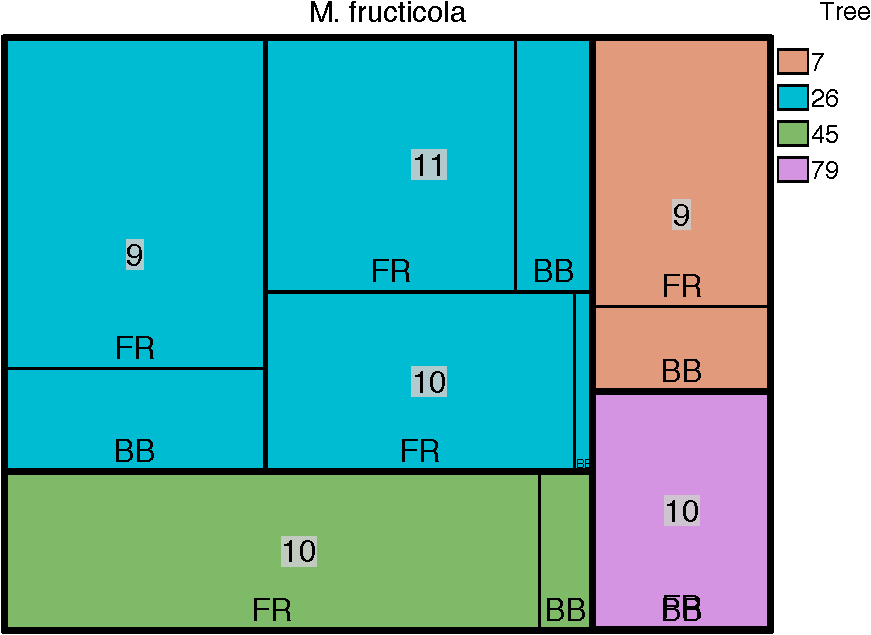
\includegraphics{_main_files/figure-latex/unnamed-chunk-9-1.pdf}

\begin{Shaded}
\begin{Highlighting}[]
\KeywordTok{itreemap}\NormalTok{(}\DataTypeTok{dtf =}\NormalTok{ monstrata, }\DataTypeTok{index =} \KeywordTok{nameStrata}\NormalTok{(monpop), }\DataTypeTok{vSize =} \StringTok{"Count"}\NormalTok{,}
        \DataTypeTok{type =} \StringTok{"categorical"}\NormalTok{, }\DataTypeTok{vColor =} \StringTok{"Tree"}\NormalTok{)}
\end{Highlighting}
\end{Shaded}

Next, we analyze the data according to Tree and Year:

\begin{Shaded}
\begin{Highlighting}[]
\KeywordTok{setPop}\NormalTok{(monpop) <-}\StringTok{ }\ErrorTok{~}\NormalTok{Tree}\OperatorTok{/}\NormalTok{Year}
\NormalTok{monpop}
\end{Highlighting}
\end{Shaded}

\begin{verbatim}
## 
## This is a genclone object
## -------------------------
## Genotype information:
## 
##    264 original multilocus genotypes 
##    694 haploid individuals
##     13 codominant loci
## 
## Population information:
## 
##      3 strata - Tree, Year, Symptom
##      6 populations defined - 7_9, 26_9, 26_10, 45_10, 79_10, 26_11
\end{verbatim}

To analyze the data according to Symptom:

\begin{Shaded}
\begin{Highlighting}[]
\KeywordTok{setPop}\NormalTok{(monpop) <-}\StringTok{ }\ErrorTok{~}\NormalTok{Symptom}
\NormalTok{monpop}
\end{Highlighting}
\end{Shaded}

\begin{verbatim}
## 
## This is a genclone object
## -------------------------
## Genotype information:
## 
##    264 original multilocus genotypes 
##    694 haploid individuals
##     13 codominant loci
## 
## Population information:
## 
##      3 strata - Tree, Year, Symptom
##      2 populations defined - BB, FR
\end{verbatim}

Order of the levels that you define is important, so if we wanted to
define the symptoms according to tree, we would use the following:

\begin{Shaded}
\begin{Highlighting}[]
\KeywordTok{setPop}\NormalTok{(monpop) <-}\StringTok{ }\ErrorTok{~}\NormalTok{Symptom}\OperatorTok{/}\NormalTok{Tree}
\NormalTok{monpop}
\end{Highlighting}
\end{Shaded}

\begin{verbatim}
## 
## This is a genclone object
## -------------------------
## Genotype information:
## 
##    264 original multilocus genotypes 
##    694 haploid individuals
##     13 codominant loci
## 
## Population information:
## 
##      3 strata - Tree, Year, Symptom
##      8 populations defined - BB_7, BB_26, FR_26, ..., BB_79, FR_79, FR_45
\end{verbatim}

Now that we have laid out the basics of manipulating data by strata, we
will now apply strata for clone correction.

Clone correction When dealing with clonal populations, analyses are
typically conducted with and without clone correction. Clone correction
is a method of censoring a data set such that only one individual per
MLG is represented per population (Milgroom, 1996; Grünwald et al.,
2003; Grünwald \& Hoheisel, 2006). This technique is commonly used with
the index of association and genotypic diversity measures since clone
corrected populations approximate behavior of sexual populations. Since
we want to only observe unique genotypes per population, clone
correction requires specification of the stratifications at which clones
should be censored. This section will show how to clone correct at a
specific stratification and also compare the results with uncorrected
data.

Question: Will allelic diversity increase or decrease with
clone-censored data? Using monpop as an example, if we wanted to know
the diversity of alleles within each tree per year, how should we go
about correcting for the clones? We use the function clonecorrect
specifying the ``Tree/Year'' strata:

\begin{Shaded}
\begin{Highlighting}[]
\NormalTok{mcc_TY <-}\StringTok{ }\KeywordTok{clonecorrect}\NormalTok{(monpop, }\DataTypeTok{strata =} \OperatorTok{~}\NormalTok{Tree}\OperatorTok{/}\NormalTok{Year, }\DataTypeTok{keep =} \DecValTok{1}\OperatorTok{:}\DecValTok{2}\NormalTok{)}
\NormalTok{mcc_TY}
\end{Highlighting}
\end{Shaded}

\begin{verbatim}
## 
## This is a genclone object
## -------------------------
## Genotype information:
## 
##    264 original multilocus genotypes 
##    278 haploid individuals
##     13 codominant loci
## 
## Population information:
## 
##      3 strata - Tree, Year, Symptom
##      6 populations defined - 7_9, 26_9, 26_10, 45_10, 79_10, 26_11
\end{verbatim}

Notice that the number of samples reduced from 694 to 278, but is still
more than the number of MLGs. This indicates that there are duplicated
genotypes that cross trees and years, but that's okay because of our
definition of a clone-corrected data set as having one representative
genotype per population. Before we continue, we should set the original
data to the same strata:

\begin{Shaded}
\begin{Highlighting}[]
\KeywordTok{setPop}\NormalTok{(monpop) <-}\StringTok{ }\ErrorTok{~}\NormalTok{Tree}\OperatorTok{/}\NormalTok{Year}
\end{Highlighting}
\end{Shaded}

Now we can compare the diversity of alleles at each locus using
Simpson's index (1−D1−D) as implemented in the function locus\_table
(Detailed in our chapter on locus based statistics). We will do this in
three steps:

Calculate diversity of the clone corrected data Calculate diversity of
the uncorrected data Take the difference of step 1 from step 2.

\begin{Shaded}
\begin{Highlighting}[]
\NormalTok{cc <-}\StringTok{ }\KeywordTok{locus_table}\NormalTok{(mcc_TY, }\DataTypeTok{info =} \OtherTok{FALSE}\NormalTok{)}
\NormalTok{mp <-}\StringTok{ }\KeywordTok{locus_table}\NormalTok{(monpop, }\DataTypeTok{info =} \OtherTok{FALSE}\NormalTok{)}
\NormalTok{mp }\OperatorTok{-}\StringTok{ }\NormalTok{cc}
\end{Highlighting}
\end{Shaded}

\begin{verbatim}
##          summary
## locus     allele      1-D     Hexp Evenness
##   CHMFc4       .  0.00158  0.00031  0.00160
##   CHMFc5       . -0.09045 -0.09114 -0.04291
##   CHMFc12      .  0.00425  0.00312  0.03873
##   SEA          .  0.03122  0.02983  0.08509
##   SED          . -0.07392 -0.07564 -0.07563
##   SEE          . -0.04693 -0.04770 -0.02642
##   SEG          .  0.03202  0.03071  0.04818
##   SEI          . -0.00902 -0.01053  0.03060
##   SEL          . -0.00919 -0.01071 -0.05397
##   SEN          . -0.05006 -0.05176 -0.07643
##   SEP          .  0.01648  0.01511  0.04087
##   SEQ          . -0.05442 -0.05620 -0.08707
##   SER          . -0.04207 -0.04374 -0.02363
##   mean         . -0.02235 -0.02372 -0.01085
\end{verbatim}

\begin{Shaded}
\begin{Highlighting}[]
\NormalTok{locus_diff <-}\StringTok{ }\NormalTok{mp }\OperatorTok{-}\StringTok{ }\NormalTok{cc}

\CommentTok{# Note that I need to select the column containing Simpson's Index. That's}
\CommentTok{# labeled as "1-D".}
\KeywordTok{barplot}\NormalTok{(locus_diff[, }\StringTok{"1-D"}\NormalTok{], }\DataTypeTok{ylab =} \StringTok{"Change in Simpson's Index"}\NormalTok{, }\DataTypeTok{xlab =} \StringTok{"Locus"}\NormalTok{,}
        \DataTypeTok{main =} \StringTok{"Comparison of clone-corrected vs. uncorrected data"}\NormalTok{)}
\end{Highlighting}
\end{Shaded}

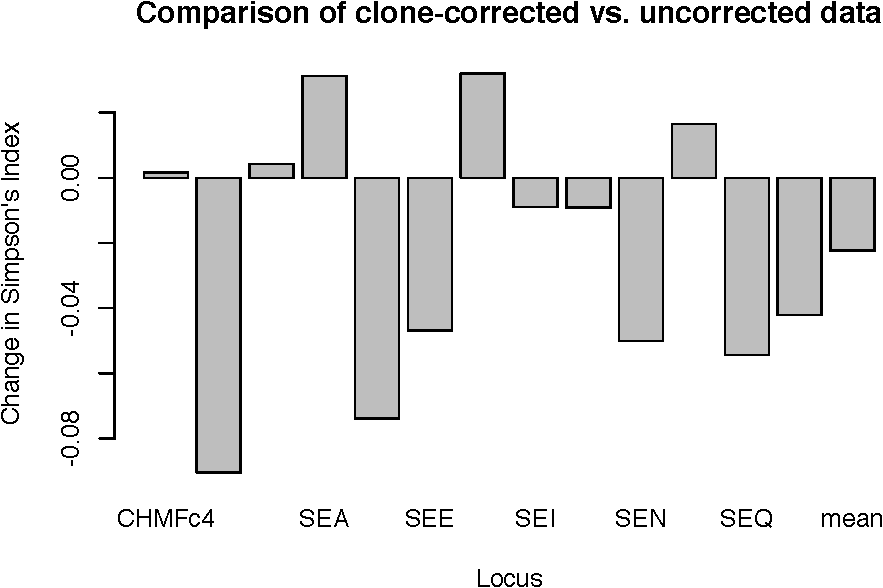
\includegraphics{_main_files/figure-latex/unnamed-chunk-17-1.pdf}

We can see quite a difference in some loci after clone correcting based
on tree in the overall data set showing that, while some loci show a
decrease, many loci show an increase in allelic diversity after
clone-correction.

Advanced R: writing your own functions for analysis by stratum Of
course, we still want to analyze each tree/year combination separately.
Instead of typing those commands above for each combination, we can
write a function to do it for us.

A function can be thought of as a set of instructions that tells the
computer what to do. You have been using functions before such as
poppr(). A function is written like this:

Writing a function for comparing clone corrected and uncorrected data

We will simply take the steps from above and turn them into a function
to calculate the difference in Simpson's diversity for a given
population. In order to do that, we will need to compute three steps:

the name of the population the clone-corrected data set the uncorrected
data set From there, we can construct the function.

\begin{Shaded}
\begin{Highlighting}[]
\NormalTok{plot_simp_diff <-}\StringTok{ }\ControlFlowTok{function}\NormalTok{(pop_name, clone_corrected, un_corrected)\{}

  \CommentTok{# Step 1: calculate diversity for clone-corrected data}
\NormalTok{  cc <-}\StringTok{ }\KeywordTok{locus_table}\NormalTok{(clone_corrected, }\DataTypeTok{pop =}\NormalTok{ pop_name, }\DataTypeTok{info =} \OtherTok{FALSE}\NormalTok{)}

  \CommentTok{# Step 2: calculate diversity for uncorrected data}
\NormalTok{  uc <-}\StringTok{ }\KeywordTok{locus_table}\NormalTok{(un_corrected, }\DataTypeTok{pop =}\NormalTok{ pop_name, }\DataTypeTok{info =} \OtherTok{FALSE}\NormalTok{)}

  \CommentTok{# Step 3: Take the difference}
\NormalTok{  res <-}\StringTok{ }\NormalTok{uc }\OperatorTok{-}\StringTok{ }\NormalTok{cc}

  \CommentTok{# Step 4: Plot Simpson's index.}
  \KeywordTok{barplot}\NormalTok{(res[, }\StringTok{"1-D"}\NormalTok{], }\DataTypeTok{main =}\NormalTok{ pop_name, }\DataTypeTok{ylab =} \StringTok{"Change in Simpson's Index"}\NormalTok{, }\DataTypeTok{xlab =} \StringTok{"Locus"}\NormalTok{)}
\NormalTok{\}}
\end{Highlighting}
\end{Shaded}

\begin{Shaded}
\begin{Highlighting}[]
\KeywordTok{par}\NormalTok{(}\DataTypeTok{mfrow =} \KeywordTok{c}\NormalTok{(}\DecValTok{2}\NormalTok{, }\DecValTok{3}\NormalTok{)) }\CommentTok{# Set up the graphics to have two rows and three columns}

\ControlFlowTok{for}\NormalTok{ (i }\ControlFlowTok{in} \KeywordTok{popNames}\NormalTok{(monpop))\{}
  \KeywordTok{plot_simp_diff}\NormalTok{(i, mcc_TY, monpop)}
\NormalTok{\}}
\end{Highlighting}
\end{Shaded}

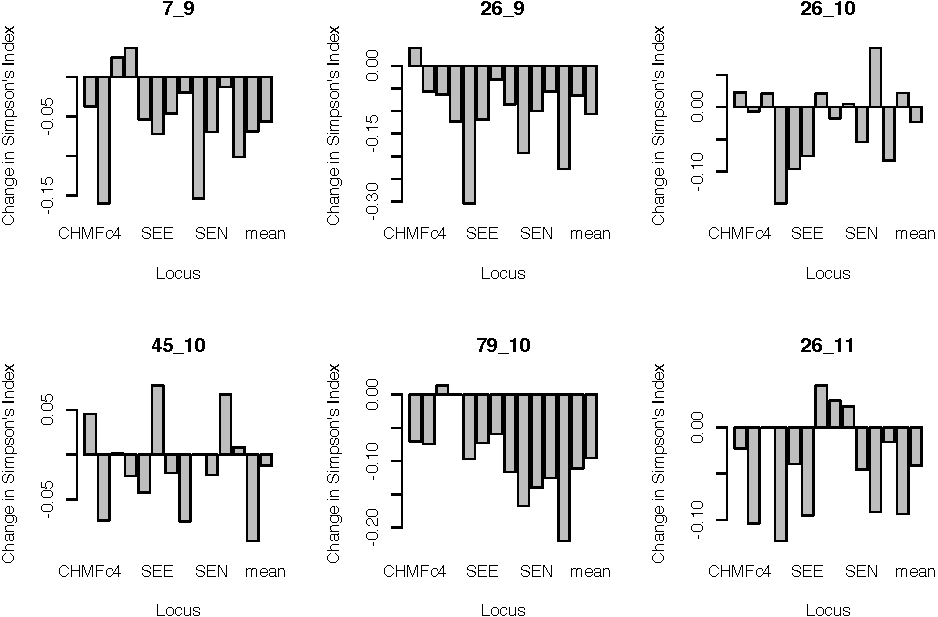
\includegraphics{_main_files/figure-latex/unnamed-chunk-19-1.pdf}

\begin{Shaded}
\begin{Highlighting}[]
\KeywordTok{par}\NormalTok{(}\DataTypeTok{mfrow =} \KeywordTok{c}\NormalTok{(}\DecValTok{1}\NormalTok{, }\DecValTok{1}\NormalTok{)) }\CommentTok{# Next we reset the graphics to have one row and one column}
\end{Highlighting}
\end{Shaded}

These barplots show the difference in Simpson's index of original minus
clone corrected data for each population per locus. We can see that
allelic diversity generally is lower in the total data set (containing
some repeated MLGs) relative to clone corrected data.

Conclusions This was a brief introduction to the easiest way to create
stratifications and apply them in poppr to more rapidly analyze your
data. By indexing the stratifications of your data, you can set the
stratification(s) you want to have analyzed in a single command. This
approach avoids having to create new sub-sets of the data for each
analysis and simultaneously reduces the chance of error when
manipulating data sets by hand.

References Everhart S., Scherm H. 2015. Fine-scale genetic structure of
Monilinia fructicola during brown rot epidemics within individual peach
tree canopies. Phytopathology 105:542--549. Available at:
\url{https://doi.org/10.1094/PHYTO-03-14-0088-R}

Grünwald NJ., Goodwin SB., Milgroom MG., Fry WE. 2003. Analysis of
genotypic diversity data for populations of microorganisms.
Phytopathology 93:738--746. Available at:
\url{http://apsjournals.apsnet.org/doi/abs/10.1094/PHYTO.2003.93.6.738}

Grünwald NJ., Hoheisel G-A. 2006. Hierarchical analysis of diversity,
selfing, and genetic differentiation in populations of the oomycete
Aphanomyces euteiches. Phytopathology 96:1134--1141. Available at:
\url{http://apsjournals.apsnet.org/doi/abs/10.1094/PHYTO-96-1134}

Milgroom MG. 1996. Recombination and the multilocus structure of fungal
populations. Annual Review of Phytopathology 34:457--477. Available at:
\url{http://www.annualreviews.org/doi/abs/10.1146/annurev.phyto.34.1.457}

Nielsen R., Slatkin M. 2013. An introduction to population genetics:
Theory and applications. Sinauer Associates, Incorporated. Available at:
\url{http://books.google.com/books?id=Iy08kgEACAAJ}

Locus stats, heterozygosity, HWE ZN Kamvar, SE Everhart, and NJ Grünwald
A rigorous population genetic analysis looks closely at the data to
assess quality and identify outliers or problems in the data such as
erroneous allele calls. This chapter focuses on analysis on a per-locus
level. While there are statistics that analyze populations across loci,
it is important to analyze each locus independently to make sure that
one locus is not introducing bias or spurious errors into the analysis.

Note: Many of these statistics are specific to co-dominant data. Locus
summary statistics A quick way to assess quality of the data is to
determine the number, diversity, expected heterozygosity, and evenness
of the alleles at each locus. As an example, we will use data for the
fungal-like protist Phytophthora infestans from (Goss et al., 2014).
First, we'll use the function locus\_table to get all of the statistics
mentioned above. For documentation on this function type ?locus\_table.
Here is a first look at each locus:

\begin{Shaded}
\begin{Highlighting}[]
\KeywordTok{library}\NormalTok{(magrittr)  }\CommentTok{# We will also use magrittr for part of this chapter}
\KeywordTok{data}\NormalTok{(Pinf)         }\CommentTok{# P. infestans data set from Mexico and South America}
\KeywordTok{locus_table}\NormalTok{(Pinf)}
\end{Highlighting}
\end{Shaded}

\begin{verbatim}
## 
## allele = Number of observed alleles
## 1-D = Simpson index
## Hexp = Nei's 1978 gene diversity
## ------------------------------------------
\end{verbatim}

\begin{verbatim}
##       summary
## locus  allele    1-D   Hexp Evenness
##   Pi02 10.000  0.633  0.637    0.663
##   D13  25.000  0.884  0.889    0.587
##   Pi33  2.000  0.012  0.012    0.322
##   Pi04  4.000  0.578  0.582    0.785
##   Pi4B  7.000  0.669  0.672    0.707
##   Pi16  6.000  0.403  0.406    0.507
##   G11  21.000  0.839  0.844    0.544
##   Pi56  3.000  0.361  0.363    0.707
##   Pi63  3.000  0.413  0.415    0.641
##   Pi70  3.000  0.279  0.281    0.580
##   Pi89 11.000  0.615  0.619    0.578
##   mean  8.636  0.517  0.520    0.602
\end{verbatim}

We can see here that we have a widely variable number of alleles per
locus and that we actually have a single locus that only has two
alleles, Pi33. This locus also has low diversity, low expected
heterozygosity and is very uneven in allele distribution. This is a sign
that this might be a phylogenetically uninformative locus, where we have
two alleles and one is occurring at a minor frequency. We will explore
analysis with and without this locus. Let's first see if both of these
alleles exist in both populations of this data set.

\begin{Shaded}
\begin{Highlighting}[]
\KeywordTok{locus_table}\NormalTok{(Pinf, }\DataTypeTok{pop =} \StringTok{"North America"}\NormalTok{)}
\end{Highlighting}
\end{Shaded}

\begin{verbatim}
## 
## allele = Number of observed alleles
## 1-D = Simpson index
## Hexp = Nei's 1978 gene diversity
## ------------------------------------------
\end{verbatim}

\begin{verbatim}
##       summary
## locus  allele    1-D   Hexp Evenness
##   Pi02  9.000  0.690  0.697    0.653
##   D13  21.000  0.895  0.906    0.684
##   Pi33  2.000  0.021  0.021    0.353
##   Pi04  4.000  0.545  0.551    0.764
##   Pi4B  5.000  0.596  0.603    0.736
##   Pi16  6.000  0.425  0.430    0.498
##   G11  15.000  0.824  0.833    0.625
##   Pi56  3.000  0.335  0.338    0.647
##   Pi63  3.000  0.310  0.313    0.568
##   Pi70  2.000  0.203  0.205    0.595
##   Pi89 11.000  0.627  0.634    0.549
##   mean  7.364  0.497  0.503    0.607
\end{verbatim}

\begin{Shaded}
\begin{Highlighting}[]
\KeywordTok{locus_table}\NormalTok{(Pinf, }\DataTypeTok{pop =} \StringTok{"South America"}\NormalTok{)}
\end{Highlighting}
\end{Shaded}

\begin{verbatim}
## 
## allele = Number of observed alleles
## 1-D = Simpson index
## Hexp = Nei's 1978 gene diversity
## ------------------------------------------
\end{verbatim}

\begin{verbatim}
##       summary
## locus  allele   1-D  Hexp Evenness
##   Pi02   5.00  0.54  0.54     0.83
##   D13   13.00  0.83  0.84     0.67
##   Pi33   1.00     .     .         
##   Pi04   4.00  0.61  0.62     0.81
##   Pi4B   7.00  0.70  0.71     0.78
##   Pi16   3.00  0.35  0.36     0.69
##   G11   14.00  0.80  0.81     0.63
##   Pi56   2.00  0.39  0.39     0.81
##   Pi63   3.00  0.50  0.51     0.73
##   Pi70   3.00  0.37  0.37     0.62
##   Pi89   2.00  0.48  0.49     0.97
##   mean   5.18  0.51  0.51     0.75
\end{verbatim}

Phylogenetically uninformative loci We can see that the South American
populations is fixed for one allele, thus it would not be a bad idea to
remove that locus from downstream analyses. We can do this using the
function informloci. This will remove loci that contain less than a
given percentage of divergent individuals (the default is 2/N2/N, where
NN equals the number of individuals in the data set).

\begin{Shaded}
\begin{Highlighting}[]
\KeywordTok{nLoc}\NormalTok{(Pinf)  }\CommentTok{# Let's look at our data set, note how many loci we have.}
\end{Highlighting}
\end{Shaded}

\begin{verbatim}
## [1] 11
\end{verbatim}

\begin{Shaded}
\begin{Highlighting}[]
\NormalTok{iPinf <-}\StringTok{ }\KeywordTok{informloci}\NormalTok{(Pinf)}
\end{Highlighting}
\end{Shaded}

\begin{verbatim}
## cutoff value: 2.32558139534884 % ( 2 samples ).
\end{verbatim}

\begin{verbatim}
## MAF         : 0.01
\end{verbatim}

\begin{verbatim}
## 
##  Found 1 uninformative locus 
##  ============================ 
##  1 locus found with a cutoff of 2 samples :
##  Pi33 
##  0 loci found with MAF < 0.01
\end{verbatim}

\begin{Shaded}
\begin{Highlighting}[]
\KeywordTok{nLoc}\NormalTok{(iPinf) }\CommentTok{# Note that we have 1 less locus}
\end{Highlighting}
\end{Shaded}

\begin{verbatim}
## [1] 10
\end{verbatim}

\begin{Shaded}
\begin{Highlighting}[]
\KeywordTok{poppr}\NormalTok{(Pinf)}
\end{Highlighting}
\end{Shaded}

\begin{verbatim}
##             Pop  N MLG eMLG    SE    H    G lambda   E.5  Hexp    Ia
## 1 South America 38  29 29.0 0.000 3.27 23.3  0.957 0.883 0.513 2.873
## 2 North America 48  43 34.5 0.989 3.69 34.9  0.971 0.871 0.503 0.223
## 3         Total 86  72 34.6 1.529 4.19 57.8  0.983 0.875 0.520 0.652
##    rbarD File
## 1 0.3446 Pinf
## 2 0.0240 Pinf
## 3 0.0717 Pinf
\end{verbatim}

\begin{Shaded}
\begin{Highlighting}[]
\KeywordTok{poppr}\NormalTok{(iPinf)}
\end{Highlighting}
\end{Shaded}

\begin{verbatim}
##             Pop  N MLG eMLG    SE    H    G lambda   E.5  Hexp    Ia
## 1 South America 38  29 29.0 0.000 3.27 23.3  0.957 0.883 0.565 2.873
## 2 North America 48  43 34.5 0.989 3.69 34.9  0.971 0.871 0.551 0.225
## 3         Total 86  72 34.6 1.529 4.19 57.8  0.983 0.875 0.571 0.655
##    rbarD  File
## 1 0.3446 iPinf
## 2 0.0255 iPinf
## 3 0.0750 iPinf
\end{verbatim}

We can see that it increased ever so slightly for the ``North America''
and ``Total'' populations, but not the ``South America'' population as
expected given the fixed alleles at locus P33.

Missing data It is often important to asses the percentage of missing
data. The poppr function info\_table will help you visualize missing
data so that you can assess how to treat these further using the
function missingno. For this example, we will use the nancycats data set
as it contains a wide variety of possibilities for missing data:

\begin{Shaded}
\begin{Highlighting}[]
\KeywordTok{data}\NormalTok{(nancycats)}
\KeywordTok{info_table}\NormalTok{(nancycats, }\DataTypeTok{plot =} \OtherTok{TRUE}\NormalTok{)}
\end{Highlighting}
\end{Shaded}

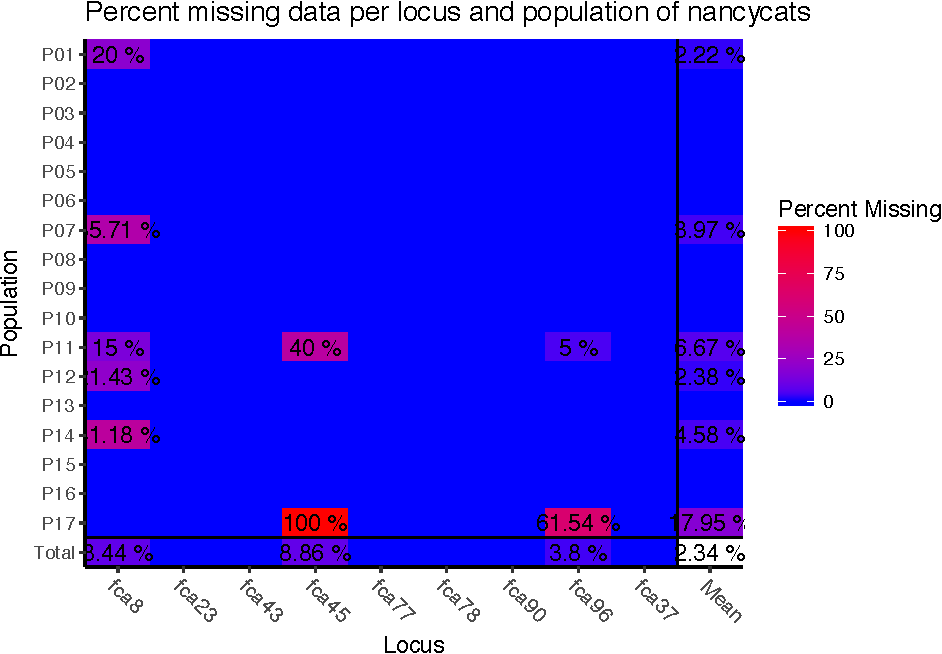
\includegraphics{_main_files/figure-latex/unnamed-chunk-23-1.pdf}

\begin{verbatim}
##           Locus
## Population  fca8 fca23 fca43 fca45 fca77 fca78 fca90 fca96 fca37  Mean
##      P01   0.200     .     .     .     .     .     .     .     . 0.022
##      P02       .     .     .     .     .     .     .     .     .     .
##      P03       .     .     .     .     .     .     .     .     .     .
##      P04       .     .     .     .     .     .     .     .     .     .
##      P05       .     .     .     .     .     .     .     .     .     .
##      P06       .     .     .     .     .     .     .     .     .     .
##      P07   0.357     .     .     .     .     .     .     .     . 0.040
##      P08       .     .     .     .     .     .     .     .     .     .
##      P09       .     .     .     .     .     .     .     .     .     .
##      P10       .     .     .     .     .     .     .     .     .     .
##      P11   0.150     .     . 0.400     .     .     . 0.050     . 0.067
##      P12   0.214     .     .     .     .     .     .     .     . 0.024
##      P13       .     .     .     .     .     .     .     .     .     .
##      P14   0.412     .     .     .     .     .     .     .     . 0.046
##      P15       .     .     .     .     .     .     .     .     .     .
##      P16       .     .     .     .     .     .     .     .     .     .
##      P17       .     .     . 1.000     .     .     . 0.615     . 0.179
##      Total 0.084     .     . 0.089     .     .     . 0.038     . 0.023
\end{verbatim}

Here we see a few things. The data set has an average of 2.34\% missing
data overall. More alarming, perhaps is the fact that population 17 has
not been genotyped at locus fca45 at all and that locus fca8 shows
missing data across many populations. Many analyses in poppr can be
performed with missing data in place as it will be either considered an
extra allele in the case of MLG calculations or will be interpolated to
not contribute to the distance measure used for the index of
association. If you want to specifically treat missing data, you can use
the function missingno to remove loci or individuals, or replace missing
data with zeroes or the average values of the locus.

Removing loci and genotypes When removing loci or genotypes, you can
specify a cutoff representing the percent missing to be removed. The
default is 0.05 (5\%).

\begin{Shaded}
\begin{Highlighting}[]
\NormalTok{nancycats }\OperatorTok\StringTok{ }\KeywordTok{missingno}\NormalTok{(}\StringTok{"loci"}\NormalTok{) }\OperatorTok\StringTok{ }\KeywordTok{info_table}\NormalTok{(}\DataTypeTok{plot =} \OtherTok{TRUE}\NormalTok{, }\DataTypeTok{scale =} \OtherTok{FALSE}\NormalTok{)}
\end{Highlighting}
\end{Shaded}

\begin{verbatim}
## 
## Found 617 missing values.
## 
## 2 loci contained missing values greater than 5%
## 
## Removing 2 loci: fca8, fca45
\end{verbatim}

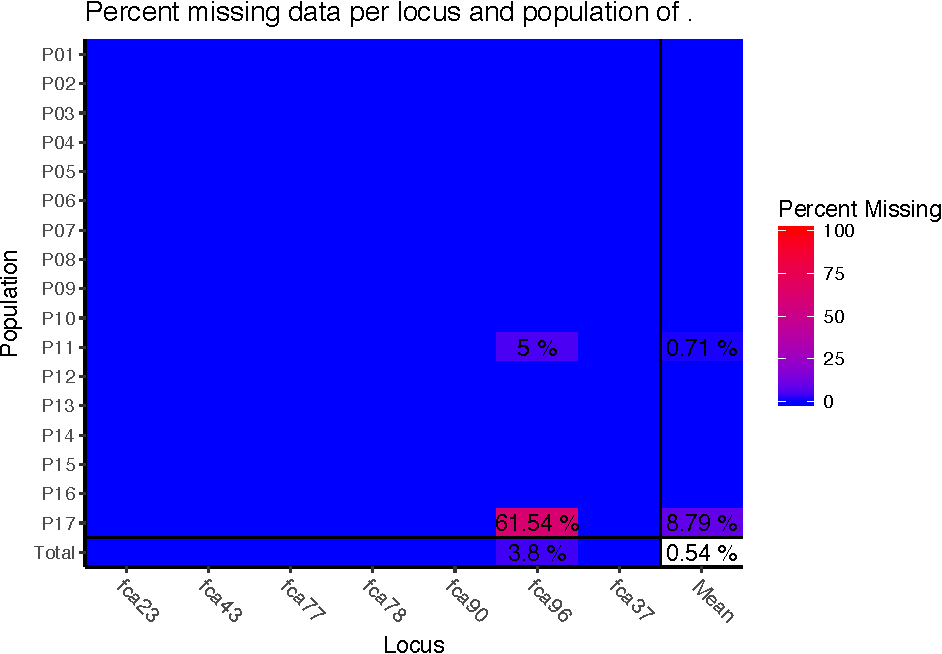
\includegraphics{_main_files/figure-latex/unnamed-chunk-24-1.pdf}

\begin{verbatim}
##           Locus
## Population fca23 fca43 fca77 fca78 fca90  fca96 fca37   Mean
##      P01       .     .     .     .     .      .     .      .
##      P02       .     .     .     .     .      .     .      .
##      P03       .     .     .     .     .      .     .      .
##      P04       .     .     .     .     .      .     .      .
##      P05       .     .     .     .     .      .     .      .
##      P06       .     .     .     .     .      .     .      .
##      P07       .     .     .     .     .      .     .      .
##      P08       .     .     .     .     .      .     .      .
##      P09       .     .     .     .     .      .     .      .
##      P10       .     .     .     .     .      .     .      .
##      P11       .     .     .     .     . 0.0500     . 0.0071
##      P12       .     .     .     .     .      .     .      .
##      P13       .     .     .     .     .      .     .      .
##      P14       .     .     .     .     .      .     .      .
##      P15       .     .     .     .     .      .     .      .
##      P16       .     .     .     .     .      .     .      .
##      P17       .     .     .     .     . 0.6154     . 0.0879
##      Total     .     .     .     .     . 0.0380     . 0.0054
\end{verbatim}

\section{Evolution of Genetic
Systems}\label{evolution-of-genetic-systems}

\section{Phylogenetics}\label{phylogenetics}

\section{Game Theory}\label{game-theory}

\section{Genetic Algorithms}\label{genetic-algorithms}

\section{Evolutionary Algorithms}\label{evolutionary-algorithms}

\section{Hardy-Weinberg}\label{hardy-weinberg}

\section{Linkage Disequilibrium}\label{linkage-disequilibrium}

\chapter{Quantitative Genetics}\label{quantitative-genetics}

\begin{itemize}
\item
  gene expression and epigenetic markers
\item
  gene-environment interaction
\end{itemize}

\url{http://nitro.biosci.arizona.edu/zbook/book.html}

\section{QTL analysis}\label{qtl-analysis}

Quantitative Trait Loci (QTL) are regions in the genome that are
associated with variation in a quantitative trait. Quantitative traits
are phentoypes that can be measured on a continuous scale, like height,
weight, etc.

QTL analysis (or QTL mapping) is typically done on experimental
populations to find genes which contribute to the heritability of
traits. Phenotype and genetic marker data are collected from every
individual in the population. The general concept of QTL mapping is that
we can then calculate the correlation between genotypes and phenotypes
at each marker position and test whether they show a statistically
significant association.

Let's consider the famous example of \citet{Doebley285}, who assessed
the variation of traits that discriminate commercial maize from its
native relative teosinte. Teosinte is much smaller than maize as we know
it today and one teosinte plant produces many ears, each of which has
only two rows of seeds. But even though maize and teosinte look so
completely different, they are still able to produce viable offspring
together. \citet{Doebley285} utilized this and crossed the two plant
species to produce an F1 generation, which were in turn self-pollinated.
The resulting F2 population of maize-teosinte-hybrids showed a wide
range of intermediate parental morphologies. Each of the F2 offspring
was then genotyped at 58 locations in the genome, so that the
quantitative trait information on morphology could be correlated with
the genetic map. This analysis revealed that most of the morphological
variation between maize and teosinte were the result of changes in only
a handful of genes, one of which is the \emph{tb1} (\emph{teosinte
branched 1}) gene.

\subsection{Recombinant Inbred Lines
(RILs)}\label{recombinant-inbred-lines-rils}

RILs are experimental sister populations that have been produced by a
very specific back-crossing scheme. The process is similar to Doebley
and Stec's crossing of maize and teosinte: two homozygous parents are
crossed to produce an F1 generation. Following the laws of genetics,
each offspring's genome consists of a random combination of parental
alleles and crossover (or recombination) events. Depending on the
design, F1 offspring are usually either selfed or mated with a sibling
to introduce another level of genetic recombination. The final
generation is then inbred for many generations to obtain a collection of
homozygous sister lines, each with a unique mosaic genome of parental
alleles \citep{Pollard2012}.

\subsection{QTL analysis in R}\label{qtl-analysis-in-r}

\subsubsection{The qtl package}\label{the-qtl-package}

The most established R package for QTL mapping is Karl Broman's
\href{http://www.rqtl.org/}{\textbf{qtl} package}\index{qtl}
\citep{R-qtl}. It implements several techniques for finding QTLs, like
Hidden Markov Models (HMM), interval mapping, Haley-Knott regression and
multiple imputation. It is very well documented and comes with extensive
example data and code.

Here, I will introduce you to a basic QTL mapping workflow using the
examples given in the package documentation and refer you to more
complex analysis options where applicable.

\paragraph{Installation and loading the
package}\label{installation-and-loading-the-package}

If this is the first time you are using the \textbf{qtl}\index{qtl}
package, you need to install it from CRAN. The following line of code
checks whether you already have the package, and if not installs it.

\begin{Shaded}
\begin{Highlighting}[]
\NormalTok{pkg =}\StringTok{ "qtl"}
\ControlFlowTok{if}\NormalTok{ (}\KeywordTok{system.file}\NormalTok{(}\DataTypeTok{package =}\NormalTok{ pkg) }\OperatorTok{==}\StringTok{ ''}\NormalTok{) }\KeywordTok{install.packages}\NormalTok{(pkg)}
\end{Highlighting}
\end{Shaded}

You can then load the package:

\begin{Shaded}
\begin{Highlighting}[]
\KeywordTok{library}\NormalTok{(qtl)}
\end{Highlighting}
\end{Shaded}

\paragraph{Loading the data}\label{loading-the-data}

I will be using the example data on murine hypertension that is provided
in the package \citep{Sugiyama200170}. In this dataset, we find
information on 250 male mice from a reciprocal backcross between two
strains: 1) the salt-sensitive C57BL/6J strain or 2) the inbred
normotensive A/J strain. These mice were then given 1\% salt water over
two weeks and their hypertension blood pressure levels were measured.

\begin{Shaded}
\begin{Highlighting}[]
\KeywordTok{data}\NormalTok{(hyper)}
\end{Highlighting}
\end{Shaded}

It is - as always - a good idea to familiarize yourself with the data to
identify potential problems or errors before spending hours or days on
an analysis that leads nowhere. The \texttt{summary()} function shows
you the main properties of the data, like number of individuals and
phenotypes, genotype information and proportion of missing data.

\begin{Shaded}
\begin{Highlighting}[]
\KeywordTok{summary}\NormalTok{(hyper)}
\end{Highlighting}
\end{Shaded}

\begin{verbatim}
##     Backcross
## 
##     No. individuals:    250 
## 
##     No. phenotypes:     2 
##     Percent phenotyped: 100 100 
## 
##     No. chromosomes:    20 
##         Autosomes:      1 2 3 4 5 6 7 8 9 10 11 12 13 14 15 16 17 18 19 
##         X chr:          X 
## 
##     Total markers:      174 
##     No. markers:        22 8 6 20 14 11 7 6 5 5 14 5 5 5 11 6 12 4 4 4 
##     Percent genotyped:  47.7 
##     Genotypes (%):    
##           Autosomes:    BB:50.1  BA:49.9 
##        X chromosome:    BY:53.0  AY:47.0
\end{verbatim}

\begin{Shaded}
\begin{Highlighting}[]
\KeywordTok{plot}\NormalTok{(hyper)}
\end{Highlighting}
\end{Shaded}

\begin{figure}
\centering
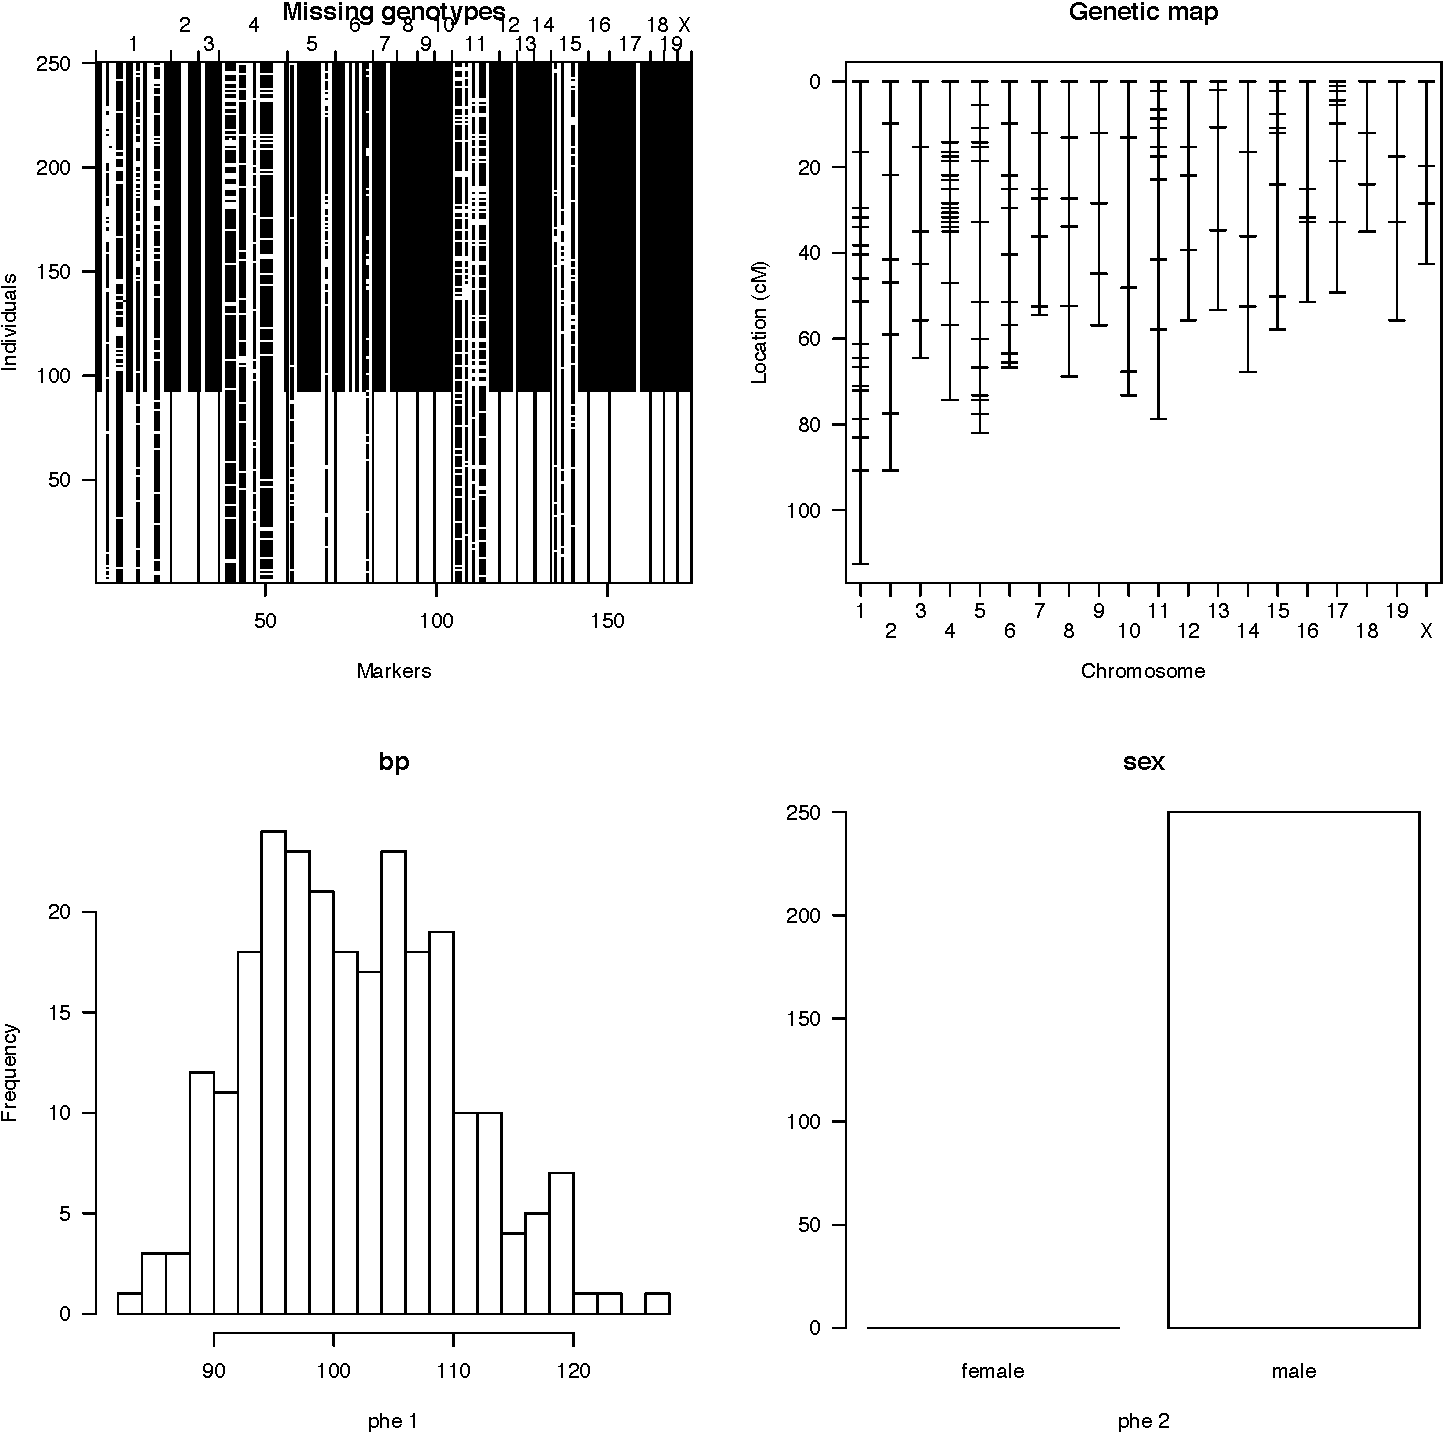
\includegraphics{_main_files/figure-latex/qtl-plot-hyper-1.pdf}
\caption{\label{fig:qtl-plot-hyper}Plots providing an overview over missing
genotypes, marker positions and the distribution of phenotypes or
traits. Plots were generated with \texttt{qtl::plot()}. In the upper
left plot markers are shown against individuals, with black areas
showing missing information. As we can see here, there is quite a bit of
missing data. The upper right plot shows the marker positions on the
chromosomes. Here, we can easily see that chromosomes 1, 4, 11 and 17
have clusters of more densely positioned markers. The lower plots show
phenotype information, either as a histogram for continuous values or as
a bar chart for categorical factors.}
\end{figure}

The \texttt{plot()} function produces plots that show missing genotypes,
marker positions and the distribution of phenotypes or traits. Figure
\ref{fig:qtl-plot-hyper} will give you a first idea about the quality of
your data.

The \href{http://www.rqtl.org/tutorials/rqtltour.pdf}{package manual}
includes a description of various additional plotting functions, which I
won't cover here.

\paragraph{Genetic map estimation}\label{genetic-map-estimation}

Before we proceed with the analysis, I typically recommend replacing the
existing genetic map with an estimated one to reduce the potential
errors. The genetic map represents all markers on a chromosome in a
linear fashion. The `est.map() function applies a Hidden Markov Model
\citep{Lander01041987} to estimate the map with an assumed genotyping
error rate (\emph{error.prob}).

Here, we can also specify the mapping function (\emph{map.function})
that we want to use to convert genetic distance to recombination
fraction. The distance between two markers is usually given as a unit of
genetic linkage, called \emph{centimorgan (cM)} One cM represents the
distance with an average of 0.01 crossover events in one generation
(i.e.~1\% recombination). However, this representation of distance
underestimates the actual recombination fraction, which is inherently
not additive. With increasing distance the chance of double crossovers
increases, so that they are in a way ``invisible'' to the traditional
estimation of recombination distance.

Another reason why genetic maps based on recombination are biased is
crossover interference, which described the phenomenon that a crossover
event reduces the likelihood of another recombination event occur close
by.

To correct for such biases, we can choose from the following mapping
functions:

\begin{itemize}
\tightlist
\item
  \textbf{Haldane's} is the simplest mapping function and assumes a
  Poisson distribution for crossover events and does not consider
  interference.
\item
  \textbf{Kosambi's} mapping function also considers interference and
  double crossovers but it can not calculate joint recombination
  probabilities for more than three loci.
\item
  \textbf{Carter-Falconer's} mapping function can be extended to more
  complex interference rates.
\item
  \textbf{Morgan's} mapping function assumes complete interference.
\end{itemize}

The two most widely used mapping functions are Haldane's (the default)
and Kosambi's. For this example, using Haldane's should be sufficient.
Because our example is a backcross, we can assume no interference,
meaning that all crossovers are independent \citep{lynch1998genetics}.

\begin{Shaded}
\begin{Highlighting}[]
\NormalTok{newmap <-}\StringTok{ }\KeywordTok{est.map}\NormalTok{(hyper, }\DataTypeTok{error.prob =} \FloatTok{0.0001}\NormalTok{, }
                  \DataTypeTok{map.function =} \StringTok{"haldane"}\NormalTok{)}
\NormalTok{hyper <-}\StringTok{ }\KeywordTok{replace.map}\NormalTok{(hyper, newmap)}
\end{Highlighting}
\end{Shaded}

We can now estimate the recombination fractions between all pairs of
markers. The \texttt{est.rf()} function also calculates the LOD scores.
LOD stands for ``likelihood of the odds'' and is a measure of linkage.
In QTL mapping we calculate LOD scores for the genetic markers and a
threshold, above which we consider a QTL statistically significant in
its association with the trait.

\begin{Shaded}
\begin{Highlighting}[]
\NormalTok{hyper <-}\StringTok{ }\KeywordTok{est.rf}\NormalTok{(hyper)}
\end{Highlighting}
\end{Shaded}

The \texttt{calc.errorlod()} function calculates the genotyping errors
according to \citet{Lincoln1992604}. We can see which markers have an
error LOD above a certain threshold (cutoff) with the
\texttt{top.errorlod()} function (Table \ref{tab:qtl-te}).

\begin{Shaded}
\begin{Highlighting}[]
\NormalTok{hyper <-}\StringTok{ }\KeywordTok{calc.errorlod}\NormalTok{(hyper, }\DataTypeTok{error.prob =} \FloatTok{0.0001}\NormalTok{)}
\NormalTok{te <-}\StringTok{ }\KeywordTok{top.errorlod}\NormalTok{(hyper, }\DataTypeTok{cutoff =} \DecValTok{3}\NormalTok{)}
\end{Highlighting}
\end{Shaded}

\begin{longtable}[]{@{}lrlr@{}}
\caption{\label{tab:qtl-te}Markers with an error LOD bigger than 3 under an
error probability of 0.0001 indicate potential genotyping
errors.}\tabularnewline
\toprule
chr & id & marker & errorlod\tabularnewline
\midrule
\endfirsthead
\toprule
chr & id & marker & errorlod\tabularnewline
\midrule
\endhead
4 & 102 & D4Mit288 & 3.324582\tabularnewline
4 & 107 & D4Mit111 & 3.262205\tabularnewline
4 & 216 & D4Mit214 & 3.261092\tabularnewline
11 & 57 & D11Mit82 & 3.021105\tabularnewline
11 & 118 & D11Mit82 & 3.021105\tabularnewline
\bottomrule
\end{longtable}

These potentially erroneous markers can then be removed or set to
\texttt{NA}.

\begin{Shaded}
\begin{Highlighting}[]
\NormalTok{hyper.clean <-}\StringTok{ }\NormalTok{hyper}
\ControlFlowTok{for}\NormalTok{ (i }\ControlFlowTok{in} \DecValTok{1}\OperatorTok{:}\KeywordTok{nrow}\NormalTok{(te)) \{}
\NormalTok{  chr <-}\StringTok{ }\NormalTok{te}\OperatorTok{$}\NormalTok{chr[i]}
\NormalTok{  id <-}\StringTok{ }\NormalTok{te}\OperatorTok{$}\NormalTok{id[i]}
\NormalTok{  mar <-}\StringTok{ }\NormalTok{te}\OperatorTok{$}\NormalTok{marker[i]}
\NormalTok{  hyper.clean}\OperatorTok{$}\NormalTok{geno[[chr]]}\OperatorTok{$}\NormalTok{data[hyper}\OperatorTok{$}\NormalTok{pheno}\OperatorTok{$}\NormalTok{id }\OperatorTok{==}\StringTok{ }\NormalTok{id, mar] <-}\StringTok{ }\OtherTok{NA}
\NormalTok{\}}
\end{Highlighting}
\end{Shaded}

\paragraph{Finding QTLs}\label{finding-qtls}

Now, we can proceed with the central step: mapping the QTLs.

Because the individuals in QTL studies are genotyped at specific marker
locations throughout the genome, we inherently have to deal with the
missing information about genotypes between markers. Hidden Markov
Models (HMM) can help us overcome this problem by calculating genotype
probabilities between markers based on the joint genotype distribution.

We first need to calculate these genotype probabilities using the
\texttt{calc.genoprob()} function. We can define several parameters,
like step size, the amount of error we want to allow for, the mapping
function and step width. Here, we want to calculate genotype
probabilities for every cM (step = 1), with a fixed step width and an
error probability of 0.0001. As above, we are again using Haldane's
mapping function.

\begin{Shaded}
\begin{Highlighting}[]
\NormalTok{hyper.clean <-}\StringTok{ }\KeywordTok{calc.genoprob}\NormalTok{(hyper.clean, }\DataTypeTok{step =} \DecValTok{1}\NormalTok{, }
                             \DataTypeTok{error.prob =} \FloatTok{0.0001}\NormalTok{, }
                             \DataTypeTok{map.function =} \StringTok{"haldane"}\NormalTok{, }
                             \DataTypeTok{stepwidth =} \StringTok{"fixed"}\NormalTok{)}
\end{Highlighting}
\end{Shaded}

The simplest QTL model, we can run is single-QTL marker regression or
interval mapping using the \texttt{scanone()} function.

These simple methods can give a good estimation of QTLs but they can
also introduce bias, especially with multiple QTL in close proximity.
More advanced mapping approaches, like Composite Interval Mapping (CIM)
are discussed later on.

The first parameter we want to specify is the phenotype(s) and model
(e.g.~parametric or non-parametric) for mapping. Here, we want to use
the first phenotype, i.e.~the first column in our phenotype matrix,
which follows a normal distribution. We can see the phenotype matrix by
calling:

\begin{Shaded}
\begin{Highlighting}[]
\NormalTok{hyper.clean}\OperatorTok{$}\NormalTok{pheno}
\end{Highlighting}
\end{Shaded}

Then, we need to specify the mapping algorithm we want to use. We can
choose from several options. Here, I will only present the practical
implications for each method. For a full discussion of the mathematical
principles, see \citet{lynch1998genetics}.

\begin{itemize}
\tightlist
\item
  \textbf{Marker regression}: Marker regression is by far the simplest
  approach to QTL mapping. Here, we calculate the association between
  phenotype and genotype at each marker position independently.
\end{itemize}

Because it is so simple, marker regression is seldom recommended to use.
With interval mapping, a phenotype \textasciitilde{} genotype
association analysis is performed for each flanking marker pair
independently. This improves the approximation and gives confidence
regions around QTL.

\begin{itemize}
\tightlist
\item
  \textbf{EM (Expectation-Maximization) algorithm}: EM is usually
  applied to maximum likelihood (ML) analyses of mixed models. It is an
  iterative process of calculating conditional probabilities and
  updating the ML estimates. This process is repeated until the
  estimates converge \citep{Lander185}. If we have a reasonably dense
  marker map, the EM algorithm will converge on the global maximum.
\item
  \textbf{(Extended) Haley-Knott regression}: Haley-Knott regression
  uses a simpler model than the EM algorithm \citep{Haley1992}. The
  extended Haley-Knott regression also considers variance is therefore
  gives improved approximations. Haley-Knott regression can give good
  approximations of the likelihood profiles for ML interval mapping but
  with more complex cases, it can be heavily biased.
\item
  \textbf{Multiple imputation}: This method uses multiple rounds of
  imputing the unknown genotypes between markers and combines them into
  a final imputation model \citep{Sen371}. This allows us to perform a
  simple analysis of variance at each position in the genome. Multiple
  imputation needs much more computational power than simpler methods
  and will usually not outperform them with single-QTL models (it is
  much more advantageous with more complex multi-QTL models, however).
\end{itemize}

Here, I will show QTL mapping examples for the EM algorithm and for
multiple imputation:

\begin{Shaded}
\begin{Highlighting}[]
\CommentTok{# EM algorithm}
\NormalTok{out.em <-}\StringTok{ }\KeywordTok{scanone}\NormalTok{(hyper.clean, }\DataTypeTok{pheno.col =} \DecValTok{1}\NormalTok{, }\DataTypeTok{model =} \StringTok{"normal"}\NormalTok{, }
                  \DataTypeTok{method =} \StringTok{"em"}\NormalTok{)}
\end{Highlighting}
\end{Shaded}

The multiple imputation method requires the use of the
\texttt{sim.geno()} function before we call the mapping function. It
calculates the joint genotype distribution based on the available marker
information and uses it to perform the imputation of missin genotypes.
With the \texttt{n.draws} parameter, we define how many imputations will
be run. The more imputations steps we run, the more precise the
genotypes but with increasing cost of computational time and power.

\begin{Shaded}
\begin{Highlighting}[]
\NormalTok{hyper.clean <-}\StringTok{ }\KeywordTok{sim.geno}\NormalTok{(hyper.clean, }\DataTypeTok{step =} \DecValTok{1}\NormalTok{, }\DataTypeTok{n.draws =} \DecValTok{100}\NormalTok{, }
                        \DataTypeTok{error.prob =} \FloatTok{0.0001}\NormalTok{, }
                        \DataTypeTok{map.function =} \StringTok{"haldane"}\NormalTok{, }
                        \DataTypeTok{stepwidth =} \StringTok{"fixed"}\NormalTok{)}

\NormalTok{out.imp <-}\StringTok{ }\KeywordTok{scanone}\NormalTok{(hyper.clean, }\DataTypeTok{pheno.col =} \DecValTok{1}\NormalTok{, }\DataTypeTok{model =} \StringTok{"normal"}\NormalTok{, }
                   \DataTypeTok{method =} \StringTok{"imp"}\NormalTok{)}
\end{Highlighting}
\end{Shaded}

Now that we have a LOD score for each marker position, we want to know
which positions are significantly associated with the phenotype. To
determine this, we will use the \textbf{scanone()} function again, but
this time we want to calculate the genome-wide LOD score threshold with
a permutation test. Above this threshold we can consider a QTL to be
statistically significant. Here, I am using a similar call as before,
but I am specifying that we want to use 1000 permutations.

\begin{Shaded}
\begin{Highlighting}[]
\NormalTok{operm.imp <-}\StringTok{ }\KeywordTok{scanone}\NormalTok{(hyper.clean, }\DataTypeTok{pheno.col =} \DecValTok{1}\NormalTok{, }\DataTypeTok{model =} \StringTok{"normal"}\NormalTok{, }
                     \DataTypeTok{method =} \StringTok{"imp"}\NormalTok{, }\DataTypeTok{n.perm =} \DecValTok{1000}\NormalTok{)}
\end{Highlighting}
\end{Shaded}

The \texttt{summary()} function will tell us our genome-wide LOD score
threshold for a given significance value (here 0.05).

\begin{Shaded}
\begin{Highlighting}[]
\NormalTok{lod <-}\StringTok{ }\KeywordTok{summary}\NormalTok{(operm.imp, }\DataTypeTok{alpha =} \FloatTok{0.05}\NormalTok{)}
\NormalTok{lod}
\end{Highlighting}
\end{Shaded}

\begin{verbatim}
## LOD thresholds (1000 permutations)
##     lod
## 5% 2.34
\end{verbatim}

And now we can also refine our QTL results by including the significance
threshold. This will give us the LOD score and estimated p-values for
each marker above the threshold, around which we can now assume to have
found a QTL for our trait of interest.

\begin{Shaded}
\begin{Highlighting}[]
\KeywordTok{summary}\NormalTok{(out.imp, }\DataTypeTok{perms =}\NormalTok{ operm.imp, }\DataTypeTok{alpha =} \FloatTok{0.05}\NormalTok{, }\DataTypeTok{pvalues =} \OtherTok{TRUE}\NormalTok{)}
\end{Highlighting}
\end{Shaded}

\begin{verbatim}
##           chr   pos  lod  pval
## c1.loc97    1 100.3 3.69 0.004
## D4Mit164    4  41.6 8.08 0.000
## D15Mit152  15  37.3 2.34 0.050
\end{verbatim}

Now that we have our QTL, we can plot them with the \texttt{plot()}
function. Here, I am plotting the results from both, the EM algorithm
and the multiple imputation method. As expected, they do not differ
much. The horizontal dotted line shows the genome-wide LOD threshold and
our two significant QTL pop up nicely on chromosomes 1 and 4.

\begin{Shaded}
\begin{Highlighting}[]
\KeywordTok{plot}\NormalTok{(out.em, }\DataTypeTok{col =} \StringTok{"blue"}\NormalTok{)}
\KeywordTok{plot}\NormalTok{(out.imp, }\DataTypeTok{col =} \StringTok{"red"}\NormalTok{, }\DataTypeTok{add =} \OtherTok{TRUE}\NormalTok{)}
\KeywordTok{abline}\NormalTok{(}\DataTypeTok{h =}\NormalTok{ lod[}\DecValTok{1}\NormalTok{], }\DataTypeTok{lty =} \DecValTok{2}\NormalTok{)}
\KeywordTok{legend}\NormalTok{(}\StringTok{"topright"}\NormalTok{, }\KeywordTok{c}\NormalTok{(}\StringTok{"EM algorithm"}\NormalTok{,}\StringTok{"Mult. imputation"}\NormalTok{), }
       \DataTypeTok{col =} \KeywordTok{c}\NormalTok{(}\StringTok{"blue"}\NormalTok{, }\StringTok{"red"}\NormalTok{), }\DataTypeTok{lty =} \DecValTok{1}\NormalTok{, }\DataTypeTok{lwd =} \DecValTok{3}\NormalTok{)}
\end{Highlighting}
\end{Shaded}

\begin{figure}
\centering
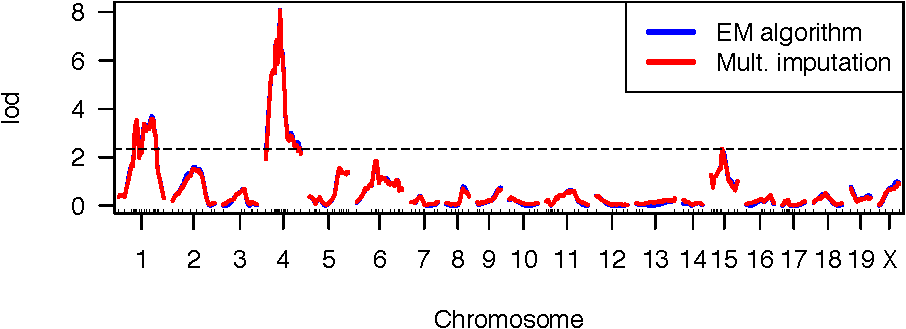
\includegraphics{_main_files/figure-latex/qtl-plot-out-1.pdf}
\caption{\label{fig:qtl-plot-out}QTL plot showing LOD scores and QTL
positions with EM algorithm and the multiple imputation. The dotted line
indicates the genome-wide LOD score threshold for a p \textless{} 0.05.
Every peak above this threshold is considered a QTL.}
\end{figure}

\paragraph{QTL interaction mapping}\label{qtl-interaction-mapping}

\paragraph{Covariates in QTL models}\label{covariates-in-qtl-models}

\subsubsection{\texorpdfstring{QTL Analysis using Bayesian Interval
Mapping (``qtlbim''
package)}{QTL Analysis using Bayesian Interval Mapping (qtlbim package)}}\label{qtl-analysis-using-bayesian-interval-mapping-qtlbim-package}

\section{Gene x Environment
interactions}\label{gene-x-environment-interactions}

\section{Variance and heritability}\label{variance-and-heritability}

\section*{Exercises: Quantitative
Genetics}\label{exercises-quantitative-genetics}


\chapter{Genetics of complex
diseases}\label{genetics-of-complex-diseases}

\section{Genome Wide Association Studies
(GWAS)}\label{genome-wide-association-studies-gwas}

\begin{itemize}
\tightlist
\item
  design and analysis of genetic association studies
\end{itemize}

\section{Pedigree analysis}\label{pedigree-analysis}

\chapter{Genetic Epidemiology}\label{genetic-epidemiology}

\section{Infection models}\label{infection-models}

\cleardoublepage 

\appendix \addcontentsline{toc}{chapter}{\appendixname}


\chapter{More to Say}\label{more-to-say}

Yeah! I have finished my book, but I have more to say about some topics.
Let me explain them in this appendix.

To know more about \textbf{bookdown}, see \url{https://bookdown.org}.

\bibliography{packages.bib,book.bib}

%\usepackage{makeidx}\makeindex
\printindex

\end{document}
